\documentclass[draft=yes,version=last,paper=a4,headings=small,titlepage,makeidx,fontsize=12pt]{scrbook} 

% ===========================================================================
% PREAMBLE
% ===========================================================================
% ===========================================================================
% PREAMBLE STANDARD (English)
% ===========================================================================
\usepackage{fontspec}%           provides font selecting commands
\usepackage{xunicode}%           provides unicode character macros
\usepackage{xltxtra} %           provides some fixes/extras
%\usepackage[utf8x]{inputenc} %  problems with xetex?
%\usepackage[utf8]{inputenc} %   problems with xetex?
%\usepackage[T1]{fontenc} %      problems with xetex and UF8?
\usepackage{tabularx}%           order matters
\usepackage{tikz}%               order matters
%\usepackage{pgf-pie} %          order matters
\usepackage{wallpaper} %         order matters
\usepackage{tabu} %              make thick lines
\usepackage{colortbl} %          make color lines
\usepackage[]{graphicx}
\usepackage{xcolor}
\usepackage{hyperref}%           configured later!
\usepackage{fullpage,longtable}% better tables
\usepackage{hhline}%             better tables
\setlength{\parindent}{0cm}
\setlength{\arrayrulewidth}{2pt}

% ===========================================================================
% SET FONTS 
%\usepackage{pifont}
%\usepackage{helvet}
\usepackage{latexsym}
\usepackage{amssymb,amsmath}

%\setmainfont{Ume Mincho S3}    % Serif      2 OK
%\setmainfont{AR PL UMing HK}   % Typewriter 1 GOOD
%\setmainfont{Sawarabi Gothic}   % SanSerif   1 GOOD
%\setmainfont{WenQuanYi Zen Hei}% SanSerif   2 OK (wrong g?)
%\setmainfont{Komatuna P}       % SanSerif   3 MAMA (but strong!)

% Should be LMRoman12 though
%\setmainfont[Mapping=tex-text]{LMRoman10}
%\setsansfont{AR PL UMing HK}
%\setmonofont{AR PL UMing HK}

%\setmainfont{IPAPMincho}
%\setmonofont{IPAPGothic}
%\setsansfont{IPAPMincho}
%\setmainfont{IPAPMincho}
%\setmonofont{IPAMincho}
%\setsansfont{IPAPMincho}

%\fontspec[
%ItalicFont={IPAGothic},
%BoldFont={IPAGothic},
%ItalicFeatures={FakeSlant},
%BoldFeatures={FakeBold=1.5},
%]{IPAPMincho}

%BoldFont = URW Palladio L, 
%ItalicFont = URW Palladio L,
%BoldItalicFont = URW Palladio L,
%SlantedFont = URW Palladio L,
%BoldSlantedFont = URW Palladio L,
%SmallCapsFont = URW Palladio L,
%UprightFont = *-Roman
%\setmainfont{YOzFontE}   % SanSerif   1 GOOD
%\setmonofont{AR PL UMing HK}

% ------  2014-09-06 -----
%\defaultfontfeatures{Ligatures=TeX}
%\setmainfont[SlantedFont={LMRoman10},
%             SlantedFeatures={FakeSlant=0.2}]{LMRoman10}
%\setsansfont[SlantedFont={LMRoman10},
%             SlantedFeatures={FakeSlant=0.2}]{LMRoman10}
\addtokomafont{footnote}{\footnotesize\sffamily}

\usepackage{array}% for vertical alignment in tabular with m{SIZE}
\usepackage{xeCJK}
\usepackage{ruby}
\renewcommand{\rubysep}{0.25ex}
\setCJKmainfont{IPAPMincho}
\setCJKfamilyfont{JapaneseDejima}{Dejima}
\setCJKfamilyfont{JapaneseYOzFont}{YOzFont90} %hand
\setCJKfamilyfont{JapaneseYOzFontA}{YOzFontA}
\setCJKfamilyfont{JapaneseYOzFontC}{YOzFontC90}
\setCJKfamilyfont{JapaneseYOzFontE}{YOzFontE90}
\setCJKfamilyfont{JapaneseYOzFontF}{YOzFontF90}
\setCJKfamilyfont{JapaneseYOzFontM}{YOzFontN90}
\setCJKfamilyfont{JapaneseYOzFontP}{YOzFontP90}
\setCJKfamilyfont{JapaneseIPAPGothic}{IPAPGothic}
\setCJKfamilyfont{JapaneseDefault}{IPAPMincho}
\newcommand\JapaneseYOzFont{\CJKfamily{JapaneseYOzFont}\CJKnospace}
\newcommand\JapaneseYOzFontA{\CJKfamily{JapaneseYOzFontA}\CJKnospace}
\newcommand\JapaneseYOzFontC{\CJKfamily{JapaneseYOzFontC}\CJKnospace}
\newcommand\JapaneseYOzFontE{\CJKfamily{JapaneseYOzFontE}\CJKnospace}
\newcommand\JapaneseYOzFontF{\CJKfamily{JapaneseYOzFontF}\CJKnospace}
\newcommand\JapaneseYOzFontM{\CJKfamily{JapaneseYOzFontM}\CJKnospace}
\newcommand\JapaneseYOzFontP{\CJKfamily{JapaneseYOzFontP}\CJKnospace}
\newcommand\JapaneseIPAPGothic{\CJKfamily{JapaneseIPAPGothic}\CJKnospace}
\newcommand\JapaneseIPAPMincho{\CJKfamily{JapaneseIPAPMincho}\CJKnospace}
\newcommand\JapaneseGothic{\CJKfamily{JapaneseIPAPGothic}\CJKnospace}
\newcommand\JapaneseDejima{\CJKfamily{JapaneseDejima}\CJKnospace}
\newcommand\JapaneseDefault{\CJKfamily{JapaneseDefault}\CJKnospace}

%\setCJKsansfont[]{}
%\setCJKmonofont[...]{...}

% Should be LMRoman12 though
%\newcommand{\Circ}[1]{\fontspec{Sawarabi Gothic}#1\setmainfont{LMRoman10}}

% ===========================================================================
% WRITE JAPANESE TEXT VERTICALLY
% derived from jltxdoc.cls and plext.dtx
%\usepackage{plext}
\def\tsample#1{%
%  \hbox to\linewidth\bgroup\vrule width.1pt\hss
  \hbox to 150mm \bgroup\vrule width.1pt\hss
    \vbox\bgroup\hrule height.1pt
      \vskip.5\baselineskip
%      \vbox to\linewidth\bgroup\tate\hsize=#1\relax\vss}
      \vbox to 150mm \bgroup\tate\hsize=#1\relax\vss}
\def\endtsample{%
      \vss\egroup
      \vskip.5\baselineskip
    \hrule height.1pt\egroup
  \hss\vrule width.1pt\egroup}

% ---------------------------------------------------------------------------
% ADD THIS PACKAGES INCASE latex AND NOT platex is used:
% \documentclass[titlepage,12pt,a4paper,german]{book}
% PAKETE
% Deutsche Umlaute etc.
% \usepackage{2up}
% \usepackage{natbib}
% \bibpunct[;]{(}{)}{;}{a}{,}{,}
% Sprache (nach natbib)
% \usepackage{babel}
% pakete aus deutscher distribution
% \usepackage{2up}


% ===========================================================================
% Better hypphenation - more space
\sloppy
\hyphenation{
bei-spiels-wei-se
chi-nesi-sche 
chi-nesi-sch-en
ein-ge-se-tzt
Ge-sell-schafts-ge-spra-che
gram-mati-schen
Ja-pa-ni-sch 
Kanji-Kana-Majiri-Bun 
Schrei-bung 
Schrift-sys-tem
Schrift-zei-chen 
}


% ===========================================================================
% PAGELAYOUT
\usepackage{geometry}
\geometry{
  top=1in,            % <-- you want to adjust this 0.5
  inner=.8in,
  outer=.6in,
  bottom=1.5in,
  footskip=5ex,   
  headheight=5ex,       % <-- and this 3
  headsep=5ex,          % <-- and this 2
}
% better head lines
\usepackage{fancyhdr}
\pagestyle{fancy}
%\fancyhead{30pt}
\setlength\headheight{25.5pt}


% ===========================================================================
% NEW DEFINITIONS FOR SYSTEM COMMANDS
\renewcommand{\chaptermark}[1]{\markboth{\textsf{\scriptsize \thechapter.\ #1\normalsize}}{}}
\renewcommand{\sectionmark}[1]{\markright{\textsf{\scriptsize\thesection.\ #1\normalsize}}{}}
 
%\renewcommand{\chaptermark}[1]{%
%\markboth{\textsf{\scriptsize \thechapter.%
%\ \chaptername:\ #1\normalsize}}{}}
%\renewcommand{\sectionmark}[1]{%
%\markright{\textsf{\scriptsize\thesection.\ #1\normalsize}}{}}

% ===========================================================================
% SETTING OWN VALUES
\setcounter{secnumdepth}{3}
\setcounter{tocdepth}{3} 
%\setlength{\baselineskip}{0pt}
%\setlength{\parskip}{\smallskipamount}
%\setlength{\parindent}{0pt}
 
% ===========================================================================
% BETTER PLACING of fig and tab ENVIRONMENTS
\usepackage{flafter}

% ===========================================================================
% LINKS
\providecolor{myblue}{rgb}{0,0.49995,1}
\hypersetup{colorlinks, 
          citecolor=myblue,
          filecolor=myblue,
          linkcolor=myblue,
          urlcolor=myblue}
% ===========================================================================
% FOR BOXES
\usepackage{microtype}
\usepackage[framemethod=TikZ]{mdframed}
\usepackage{tcolorbox}
\usepackage[tikz]{bclogo}
\usepackage{lipsum}

% ===========================================================================
% REVISION DATE VERSION
\include{VERSION}
\include{DATE}
\include{revision}

% ===========================================================================
% INDEX
\usepackage{makeidx}
\makeindex


% SIMPLE COMMANDS
\newcommand{\AuthorName}{\textsf{\LARGE Christian K{ü}lker}}

\newcommand{\NumberTwo}{%
\includegraphics[scale=0.5,trim= 00 10 00 00]{../share/i/2.eps}
}

\newcommand{\TitlePicture}{%
\begin{center}%
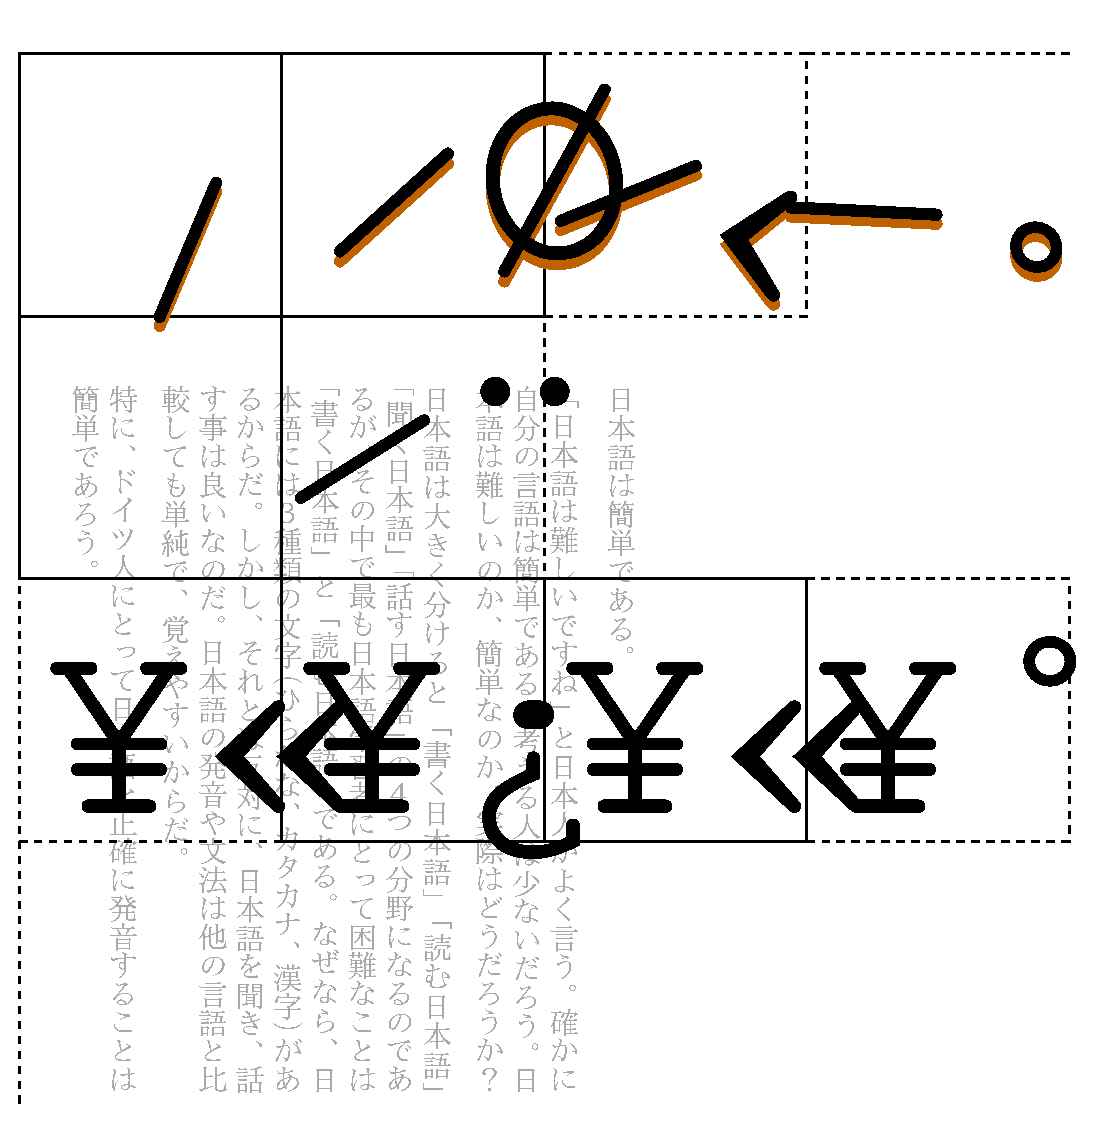
\includegraphics[scale=.5]{../share/i/kakikata-title-picture-600dpi.eps}%
\end{center}%
}%

\newcommand{\Kletter}[1]{%       l  b  r  t
\includegraphics[scale=0.95,trim=02 10 02 00,clip]{../share/katakana/#1.pdf}
}

\newcommand{\KLETTER}[1]{%
\includegraphics[scale=1.9,trim= 00 05 00 00]{../share/katakana/#1.pdf}}

\newcommand{\Link}{ {
\includegraphics[scale=0.4,trim=00 00 01 00]{../share/i/link.pdf}} }

\newcommand{\Padding}{\renewcommand*{\arraystretch}{1.4}}
  % add space between content and lines

% PARAGRAPH COMMANDS
\newcommand{\Warn}[1]{
\begin{mdframed}[
linecolor=black!40,
outerlinewidth=1pt,
roundcorner=.5em,
innertopmargin=2ex,
innerbottommargin=.5\baselineskip,
innerrightmargin=1em,
innerleftmargin=1em,
backgroundcolor=blue!10,
%userdefinedwidth=1\textwidth,
shadow=true,
shadowsize=6,
shadowcolor=black!20,
frametitle={Warning!},
frametitlebackgroundcolor=red!40,
frametitlerulewidth=10pt
]

#1

\end{mdframed}
}
 % red   - additional dangerous info reg. lang
\newcommand{\Hint}[2]{
\bigskip
\relax
\begin{mdframed}[
linecolor=black!40,
outerlinewidth=1pt,
roundcorner=.5em,
innertopmargin=2ex,
innerbottommargin=.5\baselineskip,
innerrightmargin=1em,
innerleftmargin=1em,
backgroundcolor=blue!10,
%userdefinedwidth=1\textwidth,
shadow=true,
shadowsize=6,
shadowcolor=black!20,
frametitle={#1},
frametitlebackgroundcolor=blue!40,
frametitlerulewidth=10pt
]

#2

\end{mdframed}
}
 % blue  - additional important info reg. lang
% +---------------------------------------------------------------------------+
% | Info.tex                                                                  |
% |                                                                           |
% | Prints info box                                                           |
% |                                                                           |
% | Version: 0.1.1                                                            |
% |                                                                           |
% | Changes:                                                                  |
% |                                                                           |
% | 0.1.1 2020-07-23 Christian Kuelker <c@c8i.org>                            |
% |     - Add nobreak option as 3rd parameter (prevent page break)            |
% | 0.1.0 2014-08-24 Christian Kuelker <c@c8i.org>                            |
% |     - Initial release                                                     |
% |                                                                           |
% +---------------------------------------------------------------------------+


% needspace=6em:
%   https://tex.stackexchange.com/questions/201553/forbid-page-break-after-the-title-in-mdframed
%   https://kebo.pens.ac.id/CTAN/macros/latex/contrib/mdframed/mdframed-doc-en.pdf
\newcommand{\Info}[3]{
\bigskip
\relax
\begin{mdframed}[
linecolor=black!40,
outerlinewidth=1pt,
roundcorner=.5em,
innertopmargin=2ex,
innerbottommargin=.5\baselineskip,
innerrightmargin=1em,
innerleftmargin=1em,
backgroundcolor=blue!10,
%userdefinedwidth=1\textwidth,
shadow=true,
shadowsize=6,
shadowcolor=black!20,
needspace=12em,
frametitle={#1},
frametitlebackgroundcolor=green!40,
frametitlerulewidth=10pt,
nobreak=#3
]

#2

\end{mdframed}
}
 % green - additional important info
\input{../share/box/Note} % gray  - additional info
\newcommand{\Krow}[6]{
\begin{tabular}{|c|c|c|c|c|c|}\hline
\raisebox{.25\height}{
\includegraphics[scale=1.0,trim= 00 00 00 00]{../share/katakana/#1.pdf}
}
&\KLETTER{#2}&\KLETTER{#3}&\KLETTER{#4}&\KLETTER{#5}&\KLETTER{#6}\\\hline
\end{tabular}
}
 % 6 parameters
\newcommand{\Transcribe}[4]{
\begin{center}\begin{tabular}{b{.5cm}b{3cm}b{4.5cm}b{4.5cm}} 
#1&#2&#3\rule[-10pt]{4.5cm}{.4pt}&#4\\
\end{tabular}\end{center}
}

\newenvironment{TranscribeEnv}{
\begin{minipage}{17cm}
\bigskip
\begin{center}
}{
\bigskip
\end{center}
\end{minipage}
}


\newcommand{\KatakanaSimpleTraining}[2]{

\subsection{Training #1}

Please transcribe the following words from #1:

\fbox{
\begin{TranscribeEnv}
#2
\end{TranscribeEnv}
}
}

% +---------------------------------------------------------------------------+
% | CharacterExplanation.tex                                                  |
% |                                                                           |
% | Provides a small space to comment on letters.                             |
% |                                                                           |
% | Version: 0.1.2                                                            |
% |                                                                           |
% | Changes:                                                                  |
% |                                                                           |
% | 0.1.2 2020-07-20 Christian Külker <c@c8i.org>                             |
% |     - Detokenize not needed                                               |
% |     - Fix \ifthenelse                                                     |
% |                                                                           |
% | 0.1.1 2020-07-10 Christian Külker <c@c8i.org>                             |
% |     - Change to fit Hiragana and Katakana                                 |
% |                                                                           |
% | 0.1.0 2013-09-10 Christian Külker <c@c8i.org>                             |
% |     - Initial release                                                     |
% |                                                                           |
% +---------------------------------------------------------------------------+
%
% USAGE:
%
%   \CharacterExplanation{soexplanation}{TEXT}
%
% detokenize:
% https://tex.stackexchange.com/questions/195491/ifthenelse-equal-string-comparison-fails

\newcommand{\CharacterExplanation}[2]{
    \bigskip
    \begin{tabular}{cc}
        \ifthenelse{\equal{Katakana}{\jscript}}{\raisebox{-.5\height}{\KLETTER{#1}}}{}%
        \ifthenelse{\equal{Hiragana}{\jscript}}{\raisebox{-.5\height}{\HLETTER{#1}}}{}%
        & \begin{minipage}{12.5cm}#2\end{minipage} \\
    \end{tabular}
    \bigskip
}


% PAGE COMMANDS
\newcommand{\KatakanaTraining}[1]{%

\bigskip Draw slowly, precise and try to make it beautiful. One line per day.

\begin{tabular}{|c|c|c|c|c|c|}\hline
\KLETTER{#1s}&\KLETTER{#1}&\KLETTER{#1g}&\KLETTER{ar}&\KLETTER{s}\\\hline
\KLETTER{s}&           &           &          &          \\\hline
\KLETTER{s}&           &           &          &          \\\hline
\end{tabular}

\bigskip Slowly from top to bottom. Precise and take care about the stroke
order. One column per hour, maximum four columns per day.

\begin{tabular}{|c|c|c|c|c|c|c|c|c|c|c|c|}\hline
\Kletter{s}&\Kletter{s}&\Kletter{s}&\Kletter{s}&\Kletter{s}&
\Kletter{s}&\Kletter{s}&\Kletter{s}&\Kletter{s}&\Kletter{#1}\\\hline
&&&&&&&&&\Kletter{#1g}\\\hline
&&&&&&&&&\Kletter{ad}\\\hline
&&&&&&&&&\Kletter{s}\\\hline
&&&&&&&&&\Kletter{s}\\\hline
&&&&&&&&&\Kletter{s}\\\hline
\end{tabular}
\newpage

Write faster from left to right. If one character is wrong continue with slower
speed.

\begin{tabular}{|c|c|c|c|c|c|c|c|c|c|c|c|}\hline
\Kletter{#1s}&\Kletter{#1}&\Kletter{#1g}&\Kletter{ar}&\Kletter{s}&
\Kletter{s}&\Kletter{s}&\Kletter{s}&\Kletter{s}&\Kletter{s}\\\hline
&&&&&&&&&\Kletter{s}\\\hline
&&&&&&&&&\Kletter{s}\\\hline
&&&&&&&&&\Kletter{s}\\\hline
&&&&&&&&&\Kletter{s}\\\hline
&&&&&&&&&\Kletter{s}\\\hline
\end{tabular}

\bigskip Repeat the training after a week in medium pace.

\begin{tabular}{|c|c|c|c|c|c|c|c|c|c|c|c|}\hline
\Kletter{s}&\Kletter{s}&\Kletter{s}&\Kletter{s}&\Kletter{s}&
\Kletter{s}&\Kletter{s}&\Kletter{s}&\Kletter{s}&\Kletter{#1}\\\hline
&&&&&&&&&\Kletter{#1g}\\\hline
&&&&&&&&&\Kletter{ad}\\\hline
&&&&&&&&&\Kletter{s}\\\hline
&&&&&&&&&\Kletter{s}\\\hline
&&&&&&&&&\Kletter{s}\\\hline
&&&&&&&&&\Kletter{s}\\\hline
\end{tabular}
\newpage
}

\newcommand{\KatakanaHeader}[2]{%
\begin{tabular}{clr}
\raisebox{-.5\height}{\includegraphics[scale=1.0,trim= 00 00 00 00]{../share/katakana/#1t.pdf}} &
\begin{minipage}{13cm}
#2
\end{minipage}&
\raisebox{-.4\height}{\includegraphics[scale=2.0,trim= 00 05 00 00]{../share/katakana/#1s.pdf}} 
\\
\end{tabular}
}


% TITLE
% ===========================================================================
% TITLE
% ===========================================================================
\author{\AuthorName}
\title{ \NumberTwo\\
    The Japanese Script \\ \texttt{日本語の書き方}\\
    \bigskip \large Katakana \\ \texttt{片仮名}
}
\date{ \TitlePicture \footnotesize \jdate, v-\jversion }
\dedication{to Francesco Belletti}
\uppertitleback{ \footnotesize

Copyright \copyright~ 2000, 2001, 2002, 2003, 2004, 2005, 2006, 2013, 2014 by
\href{mailto:christian.kuelker@cipworx.org}{Christian K\"ulker}.

\medskip

See the web page 
\href{http://christian.kuelker.info/nihongo/}{http://christian.kuelker.info/nihongo/}

%” ”
%"

Permission is granted to copy, distribute and/or modify this document under the
terms of the GNU Free Documentation License (GNU-FDL), version 1.2 or any later
version published by the Free Software Foundation; with no invariant sections
except the following invariant back-cover text (see framed box below:
\textit{Back-Cover Text}).

A copy of the license is included in the section entitled ”GNU Free
Documentation License”. 

\normalsize
}
\lowertitleback{     \begin{center}
        \textbf{Back-Cover Text:}
        \begin{tabular}{|l|}\hline
            \begin{minipage}{140mm}\medskip

                The original version of this book was written by
                \textbf{Christian Külker} and is copyrighted 2000-2006,
                2013-2014 under the GNU-FDL version 1.2 or any later version
                published by the Free Software Foundation with only this
                section as invariant section. \medskip

                The version v0.1 - v0.8 of this book \textbf{日本語を書こう!}
                (German: \textit{Lasst uns Japanisch schreiben!}) was developed
                as reference and training book for the language course at the
                VHS Halle (Ravensberg) in Germany starting year 2000. It was
                published 2003, 2004 and 2006 under the GNU FDL.\medskip

		In 2014 (v0.9) the part of Katakana was made a book on its own.
		The title was changed to \textbf{日本語の書き方:片仮名}
		(English: \textit{The Japanese Script - Katakana}) and adopted
		to a self study approach.\medskip

                To obtain an original copy see:
                http://christian.kuelker.info/nihongo/ For questions use
                christian.kuelker@cipworx.org.

                \flushright  Christian Külker, Tolmezzo, \jdate, v-\jversion

                \medskip

            \end{minipage}\\ \hline
        \end{tabular}
    \end{center}
    \bigskip

    \texttt{v0.9}: Initial version as Katakana only book.

    In case you have the original book, please write to
    \href{mailto:christian.kuelker@cipworx.org}{christian.kuelker@cipworx.org}
    for hints, suggestions, thanks, complains.

}


% ===========================================================================
% DOCUMENT
% ===========================================================================
\begin{document}
\fontspec{FreeSans}
\pagestyle{plain}
\frontmatter
\maketitle

% CONTENTS
\tableofcontents
\pagestyle{fancy}

\bigskip

\textbf{Conventions Used in this Document}

\bigskip

(1) The reading of Japanese characters (\hyperref[sec:Kanji]{Kanji}) are
\textbf{not} given in the section or chapter heading but as soon as possible.
If the reading is given it will be given in \hyperref[sec:Hiragana]{Hiragana}
script. To mark this reading it will start with a Japanese bracket {【} and end
with a Japanese bracket {】}.

\bigskip
\textit{Example:}

\bigskip
\begin{center}
     Kani {漢字} {【かんじ】}
\end{center}

\bigskip

(2) If readings of Japanese are also given in \hyperref[sec:Romaji]{Rōmaji}
according to the \hyperref[sec:Hepburn]{Hepburn system}. This is indicated by a
slash '/' for the beginning and a slash for the ending.

\bigskip
\textit{Example:}

\bigskip
\begin{center}
     First Katakana letter {ア} {/a/}
\end{center}

\bigskip

(3) External hyper links are marked with an arrow.

\bigskip
\textit{Example:}

\bigskip
\begin{center}
     Please look at the download page for this document, if there is a new
     version\\ \Link
     \href{http://christian.kuelker.info/nihongo}{http://christian.kuelker.info/nihongo}
\end{center}



\newpage

\Warn{Warning!}{This work is a \textbf{draft}. It is not complete and contains
errors. Please report.}

\mainmatter

\chapter*{Introduction - 前書き}

The first chapter will introduce the Japanese writing system and different
alphabets. I you are already familiar with it, you can safely skip this
chapter. In any case all terms are explained in the last chapter.

The second chapter starts with the introduction of writing and reading single
Katakana letters. The chapter ends with special Katakana letters. It is advised
to read this chapter before starting the training. 

The third chapter goes right into action by offering row based training
sessions for each character as well as simple training for writing some
Japanese Katakana words.


The last chapter provides an alphabetically ordered glossary about the most
important key words.
          % Introduction
% ===========================================================================
\chapter{Japanese Writing System - 日本語の書き方}\label{chap:JapaneseWritingSystem}

From the perspective of an European the Japanese script (how Japanese is
written) looks strange and difficult at the first sight and many people mistake
Japanese for Chinese\footnote{In German language the word "Fachchinesisch"
(Lit.: profession Chinese, Engl.: gobbledygook, Amer.: gobbledegook) for
example is synonym of something that is not understandable. The perception to
understand Japanese is almost the same.} writing. For Japanese the Japanese
script is just ordinary. On the other side the writing system of an European
language is also not easy to a Japanese. Most Japanese will not notice the
whole difficulty because they are introduced to English at an early age and
school English is just a subset of every day written English. The difficulties
starts where Japanese are exposed to every day written English or any other
European language with all it different graphical representations.

Most Europeans believe that they are using only one writing script. At a closer
look that is wrong.

\bigskip Example of 4 different representation of the reading "a":

\begin{center}
\begin{tabular}{|l|l|l|l|}
\textbf{Character}&\textbf{Alphabet}&\textbf{Reading}&\textbf{Remark}\\\hline
\textit{a}     &  Italic        & a & printed script, small letter ``a'' \\ 
\texttt{a}     &  Typewriter    & a & printed script, small letter ``a'' \\ 
A              &  Serif         & a & printed script, capital letter ``a'' \\ 
$\mathfrak{A}$ & Fraktur\footnote{Some of this writing scripts where used 
actively in the beginning of last century, while is is more common to only 
read them now.}& a & Fraktur, capital letter ``a''  \\ 
\end{tabular}
\end{center}

Some of this writing scripts where used active in the beginning of last
century, while is is more common to only read them now. 

For an European adult\footnote{European children have to learn that
"\textit{a}" is the same as "\texttt{a}". And even adults have difficulties to
read "$\mathfrak{A}$" out of context as "A".}  the "kinship" of the above
graphic elements is obvious. However it is a cultural achievement to associate
them to each other and it is by no means obvious from a foreign (or learner's)
perspective. 

In a similar way the equality of {「あ」} and {「ア」} is obvious for a
Japanese, but not for an European. When got used to it, it will become not
strange or difficult any more.

As in European text also in Japanese text a number of different scripts can be
found. Next to the known scripts in Europe\footnote{German for example:
Fraktur, Latin, special characters like umlauts or eszett (the German
symbol for a voiceless "s" after a long vowel (such as in "großer Mann") or a
diphthong (such as in "weißer Hai"). ('ß')), Indian numbers} there are two
Japanese alphabets
%\footnote{ From a scientific point of view it can be argued
%that the Roman a-z or A-Z is an \textit{alphabet} but the
%Japanese \hyperref[sec:Hiragana]{Hiragana} and \hyperref[sec:Katakana]{Katakana}
%are not. On the other side we could try to argue that a-z and A-Z are to
%different \textit{alphabets}, because the graphical representation of a sound
%is different (and alpha is Greek letter anyway). If we follow this
%argumentation we might state that \hyperref[sec:Hiragana]{Hiragana} is small
%writing while Katakana is capital writing. However both ways of argumentations
%have its short comings. By using the word \textit{alphabet}
%for \hyperref[sec:Hiragana]{Hiragana} as well as for "Typewriter" above two goals
%are in the focus of mind. First, the word \textit{alphabet} is a generic term
%for a common set of letters that is understood by everyone and second by using
%an average term for European and Japanese language the similarities should been
%stressed and not the (of course) existing differences. The friction by using
%the word \textit{alphabet} for "Typewriter" for example is well understood and
%intended. } 
 \hyperref[sec:Hiragana]{Hiragana} and
\hyperref[sec:Katakana]{Katakana}, both are referenced as \textit{Kana} and
the letters derived from Chinese characters called \hyperref[sec:Kanji]{Kanji}.

Example:

\begin{center}
\begin{tabular}{|l|l|l|l|}
\textbf{Character}&\textbf{Alphabet}&\textbf{Reading}&\textbf{Remark}\\\hline
あ& Hiragana & a & no meaning, just the letter  ``a'' in Hiragana \\
ァ& Katakana & a & no meaning, just the letter ``a'' in Katakana \\
阿& Kanji    & a & { angle, to please, part of roof, hill, Africa}\\
\end{tabular}
\end{center}

Japanese can be written in two directions. First, old fashioned from up to down
- vertically with columns from right to left. And second, modern (as in
  English) from left to right - horizontally with rows from up to down. Within
  this four alphabets are used: Roman-Indian letters (our letters),
  \hyperref[sec:Kanji]{Kanji} (Chinese derived letters)
  \hyperref[sec:Hiragana]{Hiragana} (Newer Japanese characters) and
   \hyperref[sec:Katakana]{Katakana}  (also newer Japanese characters).  This
  mixture of alphabets is named \textit{Kanji-Kana-Majiri-Bun}
  (Kanji-Kana-Mixed-Text). The most common are \hyperref[sec:Kanji]{Kanji} and
  \hyperref[sec:Hiragana]{Hiragana}. Each of the scripts are introduced in the
  following sections.

\section*{\textit{Kanji}} 
1300 years ago the first endeavours where undertaken to display the Japanese
language with the only known alphabet in the region, the Chinese writing
system. While the Japanese language where hardly suited for the writing system
it was an  economical choice since the Chinese characters where well developed
at that time and introduced many new ideas in lexis. The 'borrowing' of Chinese
characters was not a one shot operation it took centuries and more then one
attempt. This long winded process led to the fact that some characters where
imported more then once from China from different times and different regions.
And because of this one Chinese character can have more then one pronunciation.
We hope that this will consolidate over the next centuries.  Today this
imported characters are known as \textbf{Kanji} in Japan.  \textbf{Kanji} is
written \textit{Hanzi} in Chinese and referencing the character from the Han
period of China. Even though today all Chinese based characters (and even some
self invented) are referenced nowadays as \textbf{Kanji}, it does not strictly
mean that they only from the Han period.

A standard Japanese text do contain \textbf{Kanji}. To master the Japanese
language over a certain level and to be over come the problem of personal
illiteracy in Japan it is highly encouraged to learn at least 600 to 800
characters. To become fully literate member of the Japanese society 2000 to
2300 \textbf{Kanji} should be learned.

Today  \textbf{Kanji} in written Japanese language are used for substantives/
nouns, verbs, adjectives and names.


\section*{\textit{Hiragana}}
Approx. in the 9th century the \textbf{Hiragana} script - written in Japanese
as {平仮名} {【ひらがな】} - was developed by simplifying Chinese characters
used for pronunciation. The number of contemporary \textbf{Hiragana} where
reduced and today 46 are used.  \textbf{Hiragana} is a
\hyperref[sec:Mora]{morae} alphabet which is mostly constructed out of
syllables. In modern Japanese language \textbf{Hiragana} is used for
\hyperref[sec:Okurigana]{Okurigana} like  verb endings, other endings as well
as for phonetic transcription and for all other words which can or should not
be written with \hyperref[sec:Kanji]{Kanji}, except words which are written in
\hyperref[sec:Katakana]{Katakana}. In simple words: if it is not known weather
the word should be written in \hyperref[sec:Kanji]{Kanji} or
\hyperref[sec:Katakana]{Katakana} write in \textbf{Hiragana}.


\section*{\textit{Katakana}}
At the same time as \hyperref[sec:Hiragana]{Hiragana}, also \textbf{Katakana}
letters where invented by simplifying the same Chinese characters used for
pronunciation.  However the look and feel of \textbf{Katakana} is more 'square'
not so 'rounded' as \hyperref[sec:Hiragana]{Hiragana}.

\textbf{Katakana} is used today for writing words of foreign origin and for
emphasizing (in commercials or \hyperref[sec:Manga]{Manga}) as well as word in
the fauna or flora.



\section*{\textit{Roman/ Latin/ Indian-Arabic Characters}}

% ---------------------------------------------------------------------------
\ifor{Rōmaji}{ローマ字}{ろーまじ}{Rōmaji}

In temporary Japan words written in western letters become more popular and
some parts of the written language is already westernized, like (Indian/
Arabic) numbers written in horizontal text almost per default. This western
Latin letters are called \textbf{Rōmaji} and are written in Japanese as
{ローマ字} {【ろおまじ】}, even though some of them are from different origin
like Indian numbers for example.



 % Japanese Writing Japanese
\chapter{Writing Katakana - 片仮名の書き方}

The second\footnote{The first is Hiragana} Japanese Kana script a
\hyperref[sec:Mora]{mora}  based writing system is called Katakana and this is
written in Japanese as {片仮名} {【かたかな】} but sometimes also as
{カタカナ}.  It consists of a little less the 50 letters, as it is usual for
morae or \hyperref[sec:Syllable]{syllable} based systems. Katakana derived from
Chinese characters, called Kanji ( {漢字} {【かんじ】} in Japanese). All
Katakana together form a complete phonetic script.

The collection of Katakana is usually displayed in the Gojūonzu (lit. Table of
Fifty Sounds), a grid of 10x5 in which the characters are displayed. Even
though nominally the Gojūonzu is containing 50 characters the grid is not
completely occupied. Additionally there is also one character added to the
end. So with five gabs and one extra letter, the current number of Katakana is
46. If we would count also the character for doubling a vowel (which is not
displayed in the Gojūonzu) we have 47 distinct characters, still below 50. 

% アイウエオ
% カキクケコ
% サシスセソ
% タチツテト
% ナニヌネノ
% ハヒフヘホ
% マミムメモ
% ヤユヨ
% ラリルレロ
% ワヲ
% ン
\index{Katakana Gojūonzu}
\index{Katakana}
\index{Gojūon}
\index{片仮名五十音図}
\bigskip
\begin{center}
%\Huge
\Padding
%\begin{tabular}{m{1.0cm}||m{1.0cm}|m{1.0cm}|m{1.0cm}|m{1.0cm}|m{1.0cm}|}
\begin{tabular}{r||c|c|c|c|c|}
             & \textbf{a}& \textbf{i}& \textbf{u}& \textbf{e}& \textbf{o}\\ \hline \hline
\textbf{-}&ア&イ&ウ&エ&オ\\\hline 
\textbf{k}&カ&キ&ク&ケ&コ\\\hline 
\textbf{s}&サ&シ&ス&セ&ソ\\\hline 
\textbf{t}&タ&チ&ツ&テ&ト\\\hline 
\textbf{n}&ナ&ニ&ヌ&ネ&ノ\\\hline 
\textbf{h}&ハ&ヒ&フ&ヘ&ホ\\\hline 
\textbf{m}&マ&ミ&ム&メ&モ\\\hline 
\textbf{y}&ヤ&  &ユ&  &ヨ\\\hline 
\textbf{r}&ラ&リ&ル&レ&ロ\\\hline 
\textbf{w}&ワ&  &  &  &ヲ\\\hline 
\textbf{*}&ン&  &  &  &  \\\hline 
\end{tabular}
\end{center}



Even though Katakana can be used by its own to express the complete content of
the Japanese language it is almost never used as such. This is due to the fact
that the other two scripts Hiragana and Kanji exists and that there was
traditionally no space character to separate words. So a Katakana sentence with
Katakana only and no spaces is hardly understandable also due to many
homophones.  But even if there are spaced it is difficult. Therefore the letter
type boundaries of Kanji, Hirangana and Katakana are the most significant
indicator for word boundaries.

In the Japanese\footnote{Until the end of World War II Katakana was used
differently. Official documents used a mix of Kanji and Katakana in a similar
way then Hiragana and Kanji today. Katakana was used for Particles and
Okurigana.} written language Katakana has a distinct role. It serves for:

\bigskip

\begin{tabular}{rp{15cm}}
1.& writing words of foreign origin\\
2.& words that need to be emphasized\\
3. &often indicate on-yomi in dictionaries\\
4.& names of minerals \\
5.& geological names \\
6.& names of fauna (animals)\\
7.& names of flora (plants)\\
8.& partly onomatopoeias in Manga\\
9.& sounds, like animal sounds or sounds made by humans\\
10.& Telegrams (before 1988)\\
11.& banking system account names\\
12.& In literature (eg. Manga) words being spoken in a (foreign) accent or "robotic" speech\\
13. &sometimes used as Furigana\\
14. & uncommon Kanji, eg.  {皮膚科} {【ひふか】} "dermatologist" written as {皮フ科}\\
15.& computer output (in 80th, before introduction of multi byte characters)\\
16. &some personal names (especially female) (common in the past: eg. セツ (setsu))\\
\end{tabular}

\medskip

Therefore in commercials, Manga and literature describing foreign concepts
Katakana has a over proportional usage.

% ---------------------------------------------------------------------------
\section{Pronunciation and Intonation}\jsec{発音とイントネーション}\label{sec:PronunciationAndIntonation}

The pronunciation of Katakana is the same as for Hiragana. Therefore every
syllable, more precise every mora corresponds to a Katakana character and is
constructed as 'consonant' + 'vowel' with the exception of |n|. This system of
letter for each mora makes pronunciation absolutely clear with no ambiguities.
However the simplicity of Katakana does not mean that pronunciation in Japanese
is simple for English speakers as it is for Germans.  The rigid structure of
the fixed mora sound in Japanese creates the challenge of learning the proper
intonation and duration of Japanese pronunciation.

Almost each Japanese word can be chunked into morae of high and low pitch witch
is a crucial aspect of the spoken language. Compared to Chinese, Japanese
luckily have only two pitches: hi and low. Sometimes this difference can be
even important for the lexis. Homophones can have for example a difference in
pitch which make them distinguishable.  The intonation of high and low pitches
is a crucial aspect of the spoken language. One of the biggest problems for
obtaining a natural sounding pronunciation is the incorrect intonation. Many
European or American learners speak without paying attention to the correct
pitch. That makes the speech sound non-natural for Japanese. In some language
course try to let the learner memorize the natural pitch of a word or even
teach rules for memorization. While there is clearly a possibility for
linguistic rules, they are hard to remember and master. Also because they can
remember the rules it is still possible to learn the correct intonation by
resorting to language learning techniques used by infants or small children:
mimicking native Japanese speakers. Therefore it is highly advised to expose
oneself to as many Japanese spoken language as possible and to mimic it. Radio,
podcasts, drama and television to name a few. However, it is not advised to
listen too much artificial sources like anime or commercials.

\bigskip
\begin{tabular}{rl}
-&every (yes \textbf{every}) mora is pronounced with the same length\\
-&there is no short and long mora or letters\\
-&every mora has a pitch: high or low\\
-&every pitch matters\\
-&the pitch can change  sometimes with its context\\
-&the pitch can change with a dialect - however standard Japanese has well defined pitches\\
\end{tabular}

\bigskip
The pronunciation of Katakana is exactly the same as for Hiragana and most
sounds are very close to the Latin pronunciation but in general are pronounced a
little shorter without any stress. Only the /ra/ sounds, like in /ra/, /ri/, /ru/,
/re/ and /ro/ have no similarity in European languages. 


The sound of the Japanese /r/ is  neither a central nor a lateral flap, but may
vary between the two. To an English speaker, its pronunciation varies between a
flapped 'd' (as in American English buddy) and a flapped 'l'.
\href{https://en.wikipedia.org/wiki/Japanese_phonology}{(Wikipedia Japanese
Phonology)}.


The following table displays the pronunciation in the Gojūonzu.

\ien{rōmaji gojūonzu}
\ien{rōmaji}
\ien{gojūon}
\ija{ローマ字五十音図}
\ija{ローマ字}
\bigskip
\begin{center}
%\LARGE
%\Huge
\Padding
\begin{tabular}{c||c|c|c|c|c|}
&\textbf{a}&\textbf{i}&\textbf{u}&\textbf{e}&\textbf{o}\\\hline\hline
\textbf{-}&a&i&u&e&o\\\hline
\textbf{k}&ka&ki&ku&ke&ko\\\hline
\textbf{s}&sa&shi&su&se&so\\\hline
\textbf{t}&ta&chi&tsu&te&to\\\hline
\textbf{n}&na&ni&nu&ne&no\\\hline
\textbf{h}&ha&hi&fu&he&ho\\\hline
\textbf{m}&ma&mi&mu&me&mo\\\hline
\textbf{y}&ya&&yu&&yo\\\hline
\textbf{r}&ra&ri&ru&re&ro\\\hline
\textbf{w}&wa&&&&o\\\hline
\textbf{{*}}&n&&&&\\\hline
\end{tabular}
\end{center}





% ---------------------------------------------------------------------------
\section{Writing Katakana Letters}\jsec{片仮名を一つづつ書く} 
% [o] LABEL
\label{sec:WritingKatakanaLetters}
% [o] INDEX
% DESTINATION (DEF)
\ifor{Katakana}{片仮名}{かたかな}{Katakana} % TARGET

Writing \textit{Katakana words} start with writing single \textit{Katakana
letters}. Knowing the writing and reading of \textit{Katakana letters} is
essential to pronounce foreign words in Japanese correctly. And that is even
more important for learners who have good English knowledge, because it is very
tempting to pronounce English words in Japanese with original English
pronunciation, which is seldom understood\footnote{The reader might try to
order a cheeseburger at a fast food restaurant insted of a /chiizubaagaa/
(チーズバーガー).} by Japanese people who are used to their Japanese-English
pronunciation. 

By learning \textit{Katakana} the understanding of morae and syllables will
also help to improve the pronunciation and understanding of Japanese. 

\textit{Katakana} as most letters are a joint combination of strokes. For the
writing of \textit{Katakana} some rules are important, which are presented here
out of order.


\begin{description}

\item[Order:] The order of strokes is important. In section
\ref{sec:StrokeOrderMatter} on page \pageref{sec:StrokeOrderMatter} more can be
found. 

\item[Fasted Method of Writing:] Often the fastest possible method of writing
or order of strokes is the correct one.  Often from left upper corner to right
lower corner. But exceptions do exist.

\item[The characters (letters) are \textit{not} symmetric.]

\item[All characters (letters) occupy a square.]

\item[The aesthetic:] What make the character to a beautiful character? The
answer is different for each character.

Following some possibilities of rule generation for the character ``u''
 {「ウ」 }:

\bigskip \CharacterExplanation{u-guide2}{The most important feature is that the
second and third line do not align. This is not an accident.}

\bigskip \CharacterExplanation{u-guide0}{Except many
\hyperref[sec:Hiragana]{Hiragana} for some \textit{Katakana} the base line is
aligned with horizon. As with this character. }


\bigskip \CharacterExplanation{u-guide1}{Also the start (or turning) points of
all other lines are aligned vertically. Which gives this \textit{Katakana} its
unique square look.}


\bigskip \CharacterExplanation{u-guide}{All together some lines need to be
remembered to write the letter beautiful.}

\bigskip

\item[A different logic:] A little bit less the
\hyperref[sec:Hiragana]{Hiragana}, but also in \textit{Katakana} there are some
lines that do not align horizontally  or vertically. Or to say it differently
some characters are not straight on purpose.

\end{description}

On top of this the following is most likely valid: only if one can write a
letter it is (easier) possible to learn faster and memorize it.


%----------------------------------------------------------------------------
\subsection{Stroke Order Matter!}\jsubsec{書き順事項}
% [o[ LABEL 
\label{sec:StrokeOrderMatter}
% [o] INDEX

Some European individualists might ask themselves \textit{"Why do I have to
remember the order of strokes - I don't obay this in my language - and who
defined this in the first place (if not me)?"} and this seems obvious in
Europe. However some reason for order exist. 

% 書き順事項 【かきじゅんじこう】

\begin{description}

\item[1. Impression:] it makes an unprofessional impression to Japanese, if one
writes characters in the wrong order. Some laughs can be observed at least.

\item[2. Tests:]  in some tests/exams (in Japan) the order of strokes will be
tested and one gets 0 points for the wrong order. 

\item[3. Time Savings:] In the most cases the predefined order is the fastest
way to write a character. Overall once save (life) time.

\item[4. Readability:] in some cases characters become readable only (or
beautiful) if the order is correct.

\item[5. Confusion Danger:] for some characters, the order is utmost
important. If not obeyed it is very likely (ie, almost certain) that these
characters become a candidate for wrong interpretation. 

\end{description}
\normalsize

\newpage
%----------------------------------------------------------------------------
\subsection{Example /u/ }\jsubsec{{「ウ」の例} }
% [o] LABEL
\label{subsec:ExampleU}
% [o] INDEX

The \textit{Katakana} /u/ is written as {「ウ」} in Japanese. The character is
composed out of the following three components:

\bigskip 
\CharacterExplanation{uds1}{This is stroke 1}
\bigskip 
\CharacterExplanation{uds2}{This is stroke 2}
\bigskip 
\CharacterExplanation{uds3}{This is stroke 3} 

Of course the strokes need to be at the right place. So better always think or
draw a frame aound. Or even better write the strokes into a frame from the
beginning!

\bigskip 
\CharacterExplanation{udss1}{This is stroke 1 in a square frame}
\bigskip 
\CharacterExplanation{udss2}{This is stroke 2 in a square frame}
\bigskip 
\CharacterExplanation{udss3}{This is stroke 3 in a square frame} 


%\begin{center}
%\textbf{Stroke 1:} \includegraphics[trim= 00 15 00 00]{../share/katakana/uds1.pdf}
%\textbf{Stroke 2:} \includegraphics[trim= 00 15 00 00]{../share/katakana/uds2.pdf}
%\textbf{Stroke 3:} 
\includegraphics[trim= 00 15 00 00]{../share/katakana/uds3.pdf}
%\end{center}
\bigskip

This components have to be written in the above mentioned enumeration order one
after another. (The first example is without frame)

\bigskip 
\CharacterExplanation{udg1}{This is stroke 1 in context}
\bigskip 
\CharacterExplanation{udg2}{This is stroke 2 in context}
\bigskip 
\CharacterExplanation{udg3}{This is stroke 3 in context}

%\begin{center}
%\textbf{Stroke 1:} \includegraphics[trim= 00 15 00 00]{../share/katakana/udg1.pdf}
%
%\textbf{Stroke 2:} \includegraphics[trim= 00 15 00 00]{../share/katakana/udg2.pdf}
%
%\textbf{Stroke 3:} 
\includegraphics[trim= 00 15 00 00]{../share/katakana/udg3.pdf}
%\end{center}

\bigskip 
\CharacterExplanation{udgs1}{This is stroke 1 in context in a square frame}
\bigskip 
\CharacterExplanation{udgs2}{This is stroke 2 in context in a square frame}
\bigskip 
\CharacterExplanation{udgs3}{This is stroke 3 in context in a square frame}

\bigskip

In the \textit{Katakana} training section in this document the order will be
introduced as red numbers and arrows which give the approximate direction where
to place the writing device. 

%\begin{center}
% \includegraphics[trim= 00 05 00 00]{../share/katakana/us.pdf}
%\end{center}
\bigskip

\CharacterExplanation{us}{Write the first short stroke straight from up to
down. Then - and this is difficult, place the second stroke in the correct
distance from the first one. Luckily this is also a straight stroke from up to
down. }

\bigskip

Of course the perception changes if the character is written in a square.
Remember that it is better to write the character in a square, because the
correct spaces between the character and the frame also determinates its
beauty.

\bigskip

\CharacterExplanation{uss}{The first stroke in the frame is not difficult, as
mentioned before it goes from straight up to down. However the frame helps because now
we understood that it is centered. The second stroke becomes also easier in a
frame because it is written at the edge of the character. After some time and
experience this is better understood. The last stroke has to join the first and
second stroke. That is still difficult with or without a frame.}

\bigskip

%----------------------------------------------------------------------------
\subsection{Stroke Types}\jsubsec{筆画の種類}
% [o] LABEL
\label{sec:StrokeTypes}
\label{sec:Stroke}
\label{subsec:StrokeTypes}
% [o] INDEX
\ifor{stroke types}{筆画の種類}{ひっかくのしゅるい}{Strich Typen}
\ifor{stroke}{筆画}{ひっかく}{Strich}
\ifor{Hiragana}{平仮名}{ひらがな}{Hiragana}
\ifor{Kanji}{漢字}{かんじ}{Kanji}

In European language there is no idea to have different \textit{stroke} types
unless one enter the field of calligraphy. In Japanese there are different kind
of \textit{strokes}.  Most important for \hyperref[sec:Kanji]{Kanji}, second
important for \hyperref[sec:Hiragana]{Hiragana} and least important for
\textit{Katakana} since \textit{Katakana} is also used for a bold replacement.
Due to this fact the five different type of Japanese \textit{strokes}
({筆画の種類} {【ひっかくのしゅるい】}) will not repeated here. For now it is
perfectly fine to make all \textit{strokes} equally thick. 



%\input{../share/sec/WritingKatakanaSentences}
\section{Special Katakana Characters}\jsec{特別カタカナ}
% [o] LABEL
\label{sec:SpecialKatakanaCharacters}
% [o] INDEX
\ifor{special Katakana characters}{特別カタカナ}{とくべつかたかな}{Spezielle Katakana Zeichen}
\ifor{Katakana}{片仮名}{かたかな}{Katakana}
\ifor{Gojūonzu}{五十音図}{ごじゅうおんず}{50 Laute Tafel}


As mentioned before \hyperref[sec:Katakana]{Katakana} is almost like Hiragana.
This is true for the \hyperref[sec:Gojuonzu]{Gojūonzu (50 sound table)  {五十音図}
{【ごじゅうおんず】}} This section will show the special characters, some are
different from the Hiragana set.

Special in some sense are characters used for punctuation, like {「。」},
{「!」} and {「?」}.  These are similar to the western counterparts but
differ a little bit. While it is obvious for the small circle {「。」}, also
{「!」} and {「?」} differ from the western equivalent in that sense that
they are \textbf{centerd} and occupy more (white) space. This characters among
other characters are used equally among Hiragana,
\hyperref[sec:Katakana]{Katakana} and Kanji. Therefore this section will not
further mention them.

%TODO check if point changes orientation and alignment in case of changing
%writing direction. 

\subsection{Doubling Vowels in Katakana}\jsubsec{カタカナでの倍増母音}
% [o] LABEL
\label{subsec:DoublingVowelsInKatakana}
\label{subsec:DoublingVowels}
\label{sec:DoublingVowelsInKatakana}
\label{sec:DoublingVowels}
% [o] INDEX
\ifor{doubling vowels}{倍増母音}{ばいぞうぼいん}{Vokalverdopplung}
\ifor{repition mark}{繰り返し記号}{くりかえしきごう}{Wiederholungszeichen}
\ifor{Katakana}{片仮名}{かたかな}{Katakana}

% カタカナでの倍増母音 【ばいぞうぼいん】

Special \hyperref[sec:Katakana]{Katakana} characters do also exists. The most
important character is Chōon {長音} {【ちょうおん】} the plain iteration
character {「ー」}, written as a stroke. It is one of the very few which
changes orientation according the writing orientation. When writing
\hyperref[sec:Katakana]{Katakana} from left to right the iteration character is
horizontal, while writing \hyperref[sec:Katakana]{Katakana} from up to down it
is vertical. The function of this character is to double the previous mora.
This is also different from Hiragana. (For doubling als other
\hyperref[sec:Katakana]{Katakana} caracter, refere to section
\nameref{sec:Iteration} on page \pageref{sec:Iteration}.)

\bigskip

\CharacterExplanation{k-iteration-s}{In standard gothic fonts the
\hyperref[sec:Katakana]{Katakana} iteration character is just a straight line
and it is not possible to understand in which direction it has to written. }

\bigskip

\CharacterExplanation{k-iteration-sm}{However if it is written with a different
font or with a brush it is clearly visible that in horizontal writing it is
written from left to right.} 

\bigskip


%\definecolor{orange}{rgb}{1,0.5,0}
%\definecolor{mygreen}{rgb}{.2,1,.2}

\bigskip
\textit{Example:}

\bigskip

\begin{center}
\begin{tabular}{p{7cm}p{7cm}}
Katakana:&Hiragana:\\
\Huge カ\textbf{\color{magenta}ー}ド /kaado/ &\Huge か\textbf{\color{magenta}あ}ど /kaado/\\
\end{tabular}
\end{center}

\bigskip

This character is very often used and makes \hyperref[sec:Katakana]{Katakana}
for this easier then Hiragana. The long vowel ambiguity do not exist.

As mentioned above the orientation of the \hyperref[sec:Katakana]{Katakana}
iteration character changes with the direction of writing. The above example
with different writing orientation.

\medskip
\textit{Example:}

\medskip

\begin{center}
\begin{tabular}{p{3.5cm}p{3.5cm}p{3.5cm}m{3.5cm}}
horizontally&
\setCJKfamilyfont{cjk-vert}[Script=CJK,RawFeature=horizontal]{IPAPGothic}
\mbox{
\begin{minipage}{3.2cm}
\Huge カ\textbf{\color{magenta}ー}ド
\end{minipage}
}
& vertically &
%\setCJKfamilyfont{cjk-vert}[Script=CJK,RawFeature=vertical]{Kozuka Gothic Pro M}
\setCJKfamilyfont{cjk-vert}[Script=CJK,RawFeature=vertical]{IPAPGothic}
\raisebox{-.5\height}{
\mbox{
\rotatebox{-90}{
\begin{minipage}{3.2cm} \CJKfamily{cjk-vert}
\Huge カ\textbf{\color{magenta}ー}ド
\end{minipage}
}
}
}
\\
\end{tabular}
\end{center}
\medskip



\subsection{Seldom Used Katakana}\jsubsec{めったに使われない片仮名}\label{subsec:SeldomlyUsedKatakana}

% めったに使われない片仮名 【めったにつかわれないかたかな】

Even though |wo| {「ヲ」}  is part if the standard letters. But since all
particle are written in Hiragana and in this case |wo| is written {「を」} the
learning of {「ヲ」} can be skipped. Unless it is important to read old texts,
like telegrams.



       % Writing Katakana
\chapter{Katakana Training - 片仮名練習}\label{chap:KatakanaTraining}

\normalsize

Every person is learning in a different way. What works well for one does not
need to work well also for the other. Because of this an ultimate receipt to
learn Katakana can not be given here. However the introduction to this chapter
would like to try to give some  hints gathered from learning and teaching
experience. 

\begin{description}

\item[Not too less:] If one learns one character per day, it will take for
Katakana roughly 46 days.  If you restrict this to working days it will take
approximately two month. If you restrict it to a 2h lesson per week it will
take a year to learn Katakana. It is obvious that one is likely to forget the
first characters when learning the last. However, even with this method it is
not impossible, but not likely.

\item[Not too much:]  To learn Katakana in one day is unlikely possible. At
least parts will be forgotten the next day.

\end{description}

From the practice the best results have been seen when learners have tried to
learn Katkana in one to three weeks. The suggestion is to learn one line (five
characters) per day in a cumulative way. Means, repeat every day the already
learned characters and that up to 10 days until all are learned. And then
repeat this exercise until they hardly can not be forgotten any more. So for
at least 14 consecutive days without break. 

\begin{description}

\item[Develop your own style:] Learning one character at a time or a row (five
characters at a time) or learn the whole table of Katakana is possible. With
some method it can take 3 weeks or with an other method 1 week. That does not
matter. What do matter is that oneself is comfortable with the method and that
oneself extract fun out of it, even when forced to learn Katakana. Decide by
yourself how often you repeat. But decide. And write down your decision. Maybe
even plan it in your daily plan. A good practice is to learn Katakana 20 times
a day for five minutes rather then one time for three hours a day or one time a
week for 10 hours. 

\item[Search for aid:] Aid can come in may manifestations. Of course it is
useful to ask a Japanese to help. But there are many other ways for helping
yourself.  One example are flashcards. Of course it is easy to print them in
this book. However as said before: find your own way. And if you create
flashcards by yourself you already learn the content up to a certain level. 

\item[Use Squares:] Some European languages uses lines to teach letters. In
Japanese you should use a square and draw the letter in the middle. If
uncertain about the shape and orientation of the character use a square and
look at the squares filled with Katakana in this section to understand the
alignment and orientation.

\end{description}

\newpage

Here are some examples for flashcards. But feel free to invent your own.


\begin{center}
\begin{tabular}{cc}
\textbf{front site Katakana}&\textbf{back site Romaji}\\
\includegraphics[scale=1.5]{../share/i/fcar.pdf}% Romaji - Katakana
&
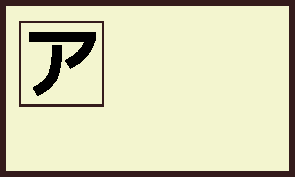
\includegraphics[scale=1.5]{../share/i/fcak.pdf}% Hiragana Katakana
\\
\end{tabular}
\end{center}

Or to learn both:

\begin{center}
\begin{tabular}{cc}
\textbf{front site Romaji}&\textbf{back site both}\\
\includegraphics[scale=1.5]{../share/i/fcar.pdf}% Romaji - Katakana
&
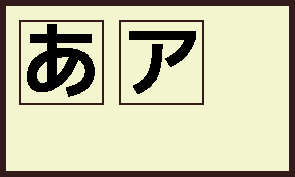
\includegraphics[scale=1.5]{../share/i/fcahk.pdf}% Hiragana Katakana
\\
\end{tabular}
\end{center}

To dive deep into Japanese of course skipping Romaji is the preferred method:

\begin{center}
\begin{tabular}{cc}
\textbf{front site Katakana}&\textbf{back site Hiragana}\\
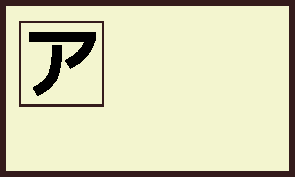
\includegraphics[scale=1.5]{../share/i/fcak.pdf}% Romaji - Katakana
&
\includegraphics[scale=1.5]{../share/i/fcah.pdf}% Hiragana Katakana
\\
\end{tabular}
\end{center}

This training chapter can be used as an additional aid to learn Katakana. And
also here it is important to develop ones own method. However some hints on
learning with this training chapter can be given.

\begin{description}

\item[Reading Loud:] While writing a Katakana character in this book (and
probably also later), read out loud the sound of the character. Always. 

\item[Invent your own cribs:] One can (maybe should?) invent one crib per
character by oneself. Especially if the characters is difficult to remember. It
might be useful to write it down on the self created flashcard for that
specific character.

\item[Regular Repetition:] It is of course possible to fill out all fields
for one chracter in a very short time. The learning effect should be minimal
though. Better is to fill out one row and then the second row an hour later,
the third row the next day and so own. Oneself has to decide the rhythm of
the repetition. 

\item[Transcription:]  Search for a  Katakana text and read it. Write for every
Katakana word the Roman letters. If this is possible without looking up the
Katakana, then the transcription should be reversed. Find some Japanese text
written in Romaji and transcribe them on Katakana on a different piece of
paper. 

\end{description}

\newpage

\section{片仮名 ア行 - Katakana |a| Row}  \label{sec:KatakanaARow}

\Krow{arow}{a}{i}{u}{e}{o}

\label{letter:a}\KLETTER{a} The 片仮名 {「ア」} derives from the
\hyperref[sec:Manyogana]{万葉仮名} characters {「阿」} left element
(\hyperref[sec:Radical]{radical}).  A smaller version {「ァ」} is used in
combinations with other letters as {「ファ」} and is pronounced as |fa| in
\hyperref[sec:Hepburn]{Hepburn} transcription.

\label{letter:u}\KLETTER{i} The 片仮名 {「イ」} derives from the
\hyperref[sec:Manyogana]{万葉仮名} characters {「伊」} left element
(\hyperref[sec:Radical]{radical}).  A smaller version {「ィ」} is used in
combinations with other letters and represents a
\hyperref[sec:Diphthong]{diphthong}. 

\label{letter:u}\KLETTER{u} The 片仮名 {「ウ」} derives from the
\hyperref[sec:Manyogana]{万葉仮名} character {「宇」}. A smaller version
{「ゥ」} is used in combinations with other letters and represents a
\hyperref[sec:Diphthong]{diphthong} and is written as "w". Even though the
combination {「トゥ」} |tu| exist, it is relatively new and many words do not
use it. In this cases {「ツ 」} |tsu| is used. {「ウ」} can take
\hyperref[sec:Dakuten]{Dakuten} to form {「ヴ」} |vu|, which is relatively new
and can replace {「ブ」} |bu|. 

\Note{Note}{%

Be aware that the characters \hyperref[letter:fu]{「フ」},
\hyperref[letter:wa]{「ワ」}  and \hyperref[letter:u]{「ウ」} look very
similar.  Make sure that you spend extra training on distinguish them. 

}%


\newpage 

\label{letter:e}\KLETTER{e} The 片仮名 {「エ」} derives from the
\hyperref[sec:Manyogana]{万葉仮名} characters {「江」} right element
(\hyperref[sec:Radical]{radical}). A smaller version {「ェ」} is used in
combinations with other letters and express \hyperref[sec:Mora]{morae} of
foreign origin. For example {「ヴェ」} as pronounced |ve|.

\label{letter:o}\KLETTER{o} The 片仮名 {「オ」} derives from the
\hyperref[sec:Manyogana]{万葉仮名} character {「於」}. A smaller version
{「ォ」} is used in combinations with other letters and express
\hyperref[sec:Mora]{morae} of foreign origin. For example {「フォ 」} as
pronounced |fe|.

\newpage


% ---------------------------------------------------------------------------
\subsection{ア - |a|} \label{sec:KatakanaA}

\KatakanaHeader{a}{ The Katakana {「ア」} is written with two strokes. The
first stroke starts horizontal. The second stroke is a curve with can be
attached to the first stroke in hand writing, but not at the horizontal part -
at the end of the first line.} \KatakanaTraining{a}

% ---------------------------------------------------------------------------
\subsection{イ - |i|} \label{sec:KatakanaI}

\KatakanaHeader{i}{ The Katakana {「イ」} is written with one stroke. The first
stroke is a curve from upper right to lower left. The second stroke is a
vertical line attached to the first at the top.} \KatakanaTraining{i}

% ---------------------------------------------------------------------------
\subsection{ウ - |u|} \label{sec:KatakanaU}

\KatakanaHeader{u}{The Katakana {「ウ」} is written with three strokes. The
first stroke a small vertical line. The second a small vertical line again and
the third line a horizontal line connection the two others.}
\KatakanaTraining{u}

% ---------------------------------------------------------------------------
\subsection{エ - |e|} \label{sec:KatakanaE}

\KatakanaHeader{e}{The Katakana {「エ」} is written with three strokes. It is
very geometrically consisting only out of horizontal and vertical lines
connected together.} \KatakanaTraining{e}

% ---------------------------------------------------------------------------
\subsection{オ - |o|} \label{sec:KatakanaO}

\KatakanaHeader{o}{The Katakana {「オ」} is written with three strokes. The
first line is horizontal and together with the second stroke it constructs a
perfect crossing. The third stroke beginning lies at the center of the
crossing.} \KatakanaTraining{o}

\section{片仮名ア行練習 -  |a| Row Training}

\KatakanaSimpleTraining{Katakana to Romaji}{
\Transcribe{1.}{ウエア}{}{wear, ware}
\Transcribe{2.}{エア}{}{air}
\Transcribe{3.}{エイ}{}{A (the letter)}
\Transcribe{4.}{アイ}{}{I (the letter)}
\Transcribe{5.}{オウ}{}{O (the letter)}
\Transcribe{6.}{イア}{}{ear}
}

\KatakanaSimpleTraining{Romaji to Katakana}{
\Transcribe{1.}{ea}{}{air}
\Transcribe{2.}{ai}{}{I (the letter)}
\Transcribe{3.}{ou}{}{O (the letter)}
\Transcribe{4.}{ei}{}{A (the letter)}
\Transcribe{5.}{uea}{}{wear, ware}
\Transcribe{6.}{ia}{}{ear}
}

\newpage

\KatakanaSimpleTraining{English to Romaji}{
\Transcribe{1.}{ear}{}{}
\Transcribe{2.}{I (the letter)}{}{}
\Transcribe{3.}{air}{}{}
\Transcribe{4.}{O (the letter)}{}{}
\Transcribe{5.}{wear, ware}{}{}
\Transcribe{6.}{A (the letter)}{}{}
}

\KatakanaSimpleTraining{English to Katakana}{
\Transcribe{2.}{I (the letter)}{}{}
\Transcribe{3.}{O (the letter)}{}{}
\Transcribe{1.}{air}{}{}
\Transcribe{6.}{ear}{}{}
\Transcribe{5.}{wear, ware}{}{}
\Transcribe{4.}{A (the letter)}{}{}
}
\newpage
   % OK
% ---------------------------------------------------------------------------
\section{Katakana /ka/ Row}\jsec{片仮名 カ行}\label{sec:KatakanaKaRow}

\Krow{karow}{ka}{ki}{ku}{ke}{ko}

\label{letter:ka}\KLETTER{ka} The  片仮名 {「カ」} is pronounced  /ka/ and  derives from the
\hyperref[sec:PhoneticCharacter]{Phonetic Character}s {「加」} left
\hyperref[sec:Radical]{radical}.  A \hyperref[sec:Dakuten]{濁点} version exists
and pronounced as /ga/.

%\hyperref[sec:Handakuten]{半濁点} does not exist in daily Japanese.  
% {「一ヵ所」} {【いちかしょ】} (one place)
% {「一ヶ所」} {【いちかしょ】} (one place).
% 十ヵ条(十ヶ条)


\Note{Note}{A smaller version {「ヵ」} is rare but used in combinations with
number particles.  For example in {「一ヵ月」} {【いっかげつ】} (one month) and
others.  This cases can also be written {「一ヶ月」} {【いっかげつ】} (one
month). Please see also \nameref{sec:KatakanaKe}. \Link
\href{http://ja.wikipedia.org/wiki/\%E3\%83\%B5}{ヵ} }

\label{letter:ki}\KLETTER{ki} The 片仮名 {「キ」} derives from the
\hyperref[sec:PhoneticCharacter]{Phonetic Character}s middle part of either {「機」} or
{「幾」}.  It is pronounced as /ki/.  A \hyperref[sec:Dakuten]{濁点} version
exists and pronounced as /gi/.


\label{letter:ku}\KLETTER{ku} The 片仮名 {「ク」} derives from the
\hyperref[sec:PhoneticCharacter]{Phonetic Character}s left upper part of {「久」}.  It
is pronounced as /ku/.  A \hyperref[sec:Dakuten]{濁点} version exists and
pronounced as /gu/.  A smaller version exists, but is used for the Ainu
Language.



\label{letter:ke}\KLETTER{ke} The 片仮名 {「ケ」} derives from the
\hyperref[sec:PhoneticCharacter]{Phonetic Character}s upper and left part of {「介」}.
It is pronounced as /ke/.  A \hyperref[sec:Dakuten]{濁点} version exists and
pronounced as /ge/.  The smaller version {「ヶ」} is explained in the following
note.

\newpage

\Note{Note}{ A smaller version {「ヶ」} is rare but used in combinations with
number particles.  For example in {「一ヶ月」} {【いっかげつ】} (one month) and
others.  This cases can also be written {「一ヵ月」} {【いっかげつ】} (one
month). There are cases where only {「ヶ」} can be written {七ヶ宿}
{【シチカシュク】} (Place at the south west border of the prefecture Miyagi).
In other rare cases this character can be pronounced different {「関ヶ原」}
{【せきがはら】} (Place at the south border of the Gifu prefecture, known by
the battle at 1600.). Please see also \nameref{sec:KatakanaKa}. \Link
\href{http://ja.wikipedia.org/wiki/\%E3\%83\%B5}{ヵ} }

\label{letter:ko}\KLETTER{ko} The 片仮名 {「コ」} derives from the
\hyperref[sec:PhoneticCharacter]{Phonetic Character}s upper part of {「己」}.  It is
pronounced as /ko/.  A \hyperref[sec:Dakuten]{濁点} version exists and
pronounced as /go/.



\newpage

% ---------------------------------------------------------------------------
\subsection{/ka/}\jsubsec{「カ」} \label{sec:KatakanaKa}

\KatakanaHeader{ka}{ /ka/ is written with 2 strokes. Basically the same way as
the Hiragana {「か」} it looks like a squarish version, but without the last
stroke. The hook at the second stroke is less significant or important.  }
\KatakanaTraining{ka}

% ---------------------------------------------------------------------------
\subsection{/ki/}\jsubsec{「キ」} \label{sec:KatakanaKi}

\KatakanaHeader{ki}{ The shape alignment of the 「キ」character is not straight
towards its environment. However the junctions are more or less 90 degrees.  }
\KatakanaTraining{ki}

% ---------------------------------------------------------------------------
\subsection{/ku/}\jsubsec{「ク」} \label{sec:KatakanaKu}
% ---------------------------------------------------------------------------

\KatakanaHeader{ku}{ The first stroke is similar the stroke of {「ケ 」} is a
curve. While the second stroke start aligned and straight. }
\KatakanaTraining{ku}

% ---------------------------------------------------------------------------
\subsection{/ke/}\jsubsec{「ケ」} \label{sec:KatakanaKe}

\KatakanaHeader{ke}{ The {「ケ 」} is written with 3 strokes and the first
stroke is similar to the {「ク」}. The second stroke is aligned and straight.
While the last stroke is a curve.  } \KatakanaTraining{ke}

% ---------------------------------------------------------------------------
\subsection{/ko/}\jsubsec{「コ」} \label{sec:KatakanaKo}

\KatakanaHeader{ko}{ This character is almost a geometric figure composed out
of two strokes. However unless in European languages this are only 2 strokes
and not 3. The first stroke is the longest one and done similar with all
{漢字}. } \KatakanaTraining{ko}

% ---------------------------------------------------------------------------
\subsection{/ka/ Row Training}\jsubsec{片仮名カ行練習}

\Padding
\begin{longtable}[c]{p{2cm}p{1.5cm}p{1.5cm}p{3cm}p{7cm}}
\textit{Katakana}&\textit{Rōmaji}&\textit{Original}&\textit{Remark}&Origin\\\hline
カキ  &kaki &kaki &柿 persimon&Japanese\\
ケア  &kea  &care &          &English\\
ケイ  &kei  &K    &the letter&English\\
\end{longtable}

\KatakanaSimpleTraining{Katakana to Rōmaji}{
\Transcribe{1.}{カキ}{}{persimmon}
\Transcribe{2.}{ココア}{}{cocoa}
\Transcribe{3.}{ケア}{}{care}
\Transcribe{4.}{コア}{}{core}
\Transcribe{5.}{ケーキ}{}{cake}
%\Transcribe{6.}{ケイ}{}{K (the letter)}
}

\KatakanaSimpleTraining{Rōmaji to Katakana}{
\Transcribe{1.}{kokoa}{}{cocoa}
\Transcribe{2.}{k$\overline{\mbox{e}}$ki}{}{cake}
\Transcribe{3.}{kea}{}{care}
\Transcribe{4.}{koa}{}{core}
\Transcribe{5.}{kaki}{}{persimmon}
%\Transcribe{6.}{kei}{}{K (the letter)}
}

\newpage

\Padding
%\begin{longtable}[c]{p{2cm}p{2cm}p{3cm}p{6cm}p{2cm}}
\begin{longtable}[c]{p{2cm}p{2.0cm}p{3.5cm}p{4cm}p{2.5cm}}
\textit{Katakana}&\textit{Rōmaji}&\textit{Original}&\textit{Remark}&Origin\\\hline
コア  &koa  &core &          &English\\
ココア&kokoa&cocoa& hot chocolate &English, from metathesis of Spanish cacao, from Nahuatl cacahuatl\\
ケーキ&kēki &cake &          &English\\
\end{longtable}


\KatakanaSimpleTraining{English to Rōmaji}{
\Transcribe{1.}{persimon}{}{}
\Transcribe{2.}{cocoa}{}{}
\Transcribe{3.}{care}{}{}
\Transcribe{4.}{core}{}{}
\Transcribe{5.}{K (the letter)}{}{}
%\Transcribe{6.}{cake}{}{}
}

\KatakanaSimpleTraining{English to Katakana}{
\Transcribe{1.}{cocoa}{}{}
\Transcribe{2.}{cake}{}{}
\Transcribe{3.}{care}{}{}
\Transcribe{4.}{persimon}{}{}
\Transcribe{5.}{K (the letter)}{}{}
%\Transcribe{6.}{core}{}{}
}

\newpage
  % OK
\section{片仮名  サ行 - Katakana |sa| Row} \label{sec:KatakanaSaRow}

\Krow{sarow}{sa}{shi}{su}{se}{so}

\KLETTER{sa} The  片仮名 {「サ」} is pronounced  |sa| and  derives from the
\hyperref[sec:Manyogana]{万葉仮名} characters {「散」} upper left corner
\hyperref[sec:Radical]{radical}.  A \hyperref[sec:Dakuten]{濁点} version exists
and pronounced as |za|.

\KLETTER{shi} The 片仮名 {「シ」} derives from the
\hyperref[sec:Manyogana]{万葉仮名} character  {「之 」}.  It is pronounced as
|shi|.  A \hyperref[sec:Dakuten]{濁点} version exists and pronounced as |ji|.

\Note{Note}{Please see section \nameref{subsec:ShiTsuAmbiguity} for the
explanation how to write and distinguish |shi| and |tsu|.  }

\KLETTER{su} The 片仮名 {「ス」} derives from the
\hyperref[sec:Manyogana]{万葉仮名} characters right lower part of {「須」}.  It
is pronounced as |su|.  A \hyperref[sec:Dakuten]{濁点} version exists and
pronounced as |zu|. 

\KLETTER{se} The 片仮名 {「セ」} derives from the
\hyperref[sec:Manyogana]{万葉仮名} characters middle left part of {「世」}.
It is pronounced as |se|.  A \hyperref[sec:Dakuten]{濁点} version exists and
pronounced as |ze|.  

\newpage

\KLETTER{so} The 片仮名 {「ソ」} derives from the
\hyperref[sec:Manyogana]{万葉仮名} characters upper right part of {「曽」}.  It is
pronounced as |so|.  A \hyperref[sec:Dakuten]{濁点} version exists and
pronounced as |zo|.

% SoRiNAmbiguity
\subsection{|so|, |ri| and |n| Ambiguity} \label{subsec:SoRiNAmbiguity}

The Katakana characters {「ソ」}, {「リ」} and {「ン」} can be difficult to
distinguish. All three are made out of only 2 strokes. And especially |so| and
|n| can be hard to tell. In a sentence of course the context can help a lot.
But what are the rules for this characters to write properly and distinguish?

\bigskip

\begin{center}
\begin{tabular}{|c|c|c|}\hline
\KLETTER{so}&\KLETTER{n}&\KLETTER{ri}\\\hline
\end{tabular}
\end{center}

\CharacterExplanation{soexplanation}{ To write the letter |so| it is important
to align both lines \textbf{horizontally} (red line) and to \textbf{non-align}
the ends (blue line).  In this way it is possible to distinguish |so| from |n|,
but not from |ri|. To also distinguish it from |ri| you have to write the first
stroke not horizontally nor vertically.  }

\CharacterExplanation{nexplanation}{ To write the letter |n| it is important to
a align both lines \textbf{vertically} (red line) and to \textbf{non-align} the
ends (blue line). In this way it is possible to distinguish |n| from |so|. If
both lines are aligned there should not be a problem to distinguish it from
|ri|.  }

\CharacterExplanation{riexplanation}{ To write the letter |ri| it is important
to a align both lines \textbf{vertically} (red line) and to \textbf{non-align}
the ends (blue line). The difference between |so| and |ri| is that |ri| need to
start with two \textbf{parallel} lines wile |so| does not. Please see green
lines for explanation.  }




\newpage

\subsection{サ - |sa|} \label{sec:KatakanaSa}

\KatakanaHeader{sa}{ Katakana {「サ」} is written with three strokes. All
crossings of strokes are in a 90 degree angle.  The starts of all strokes are
aligned eitehr horizontally or vertically. The last stroke has a curve.}
\KatakanaTraining{sa}

\subsection{シ - |shi|} \label{sec:KatakanaShi}

\KatakanaHeader{shi}{ The Katakana {「シ」} is written with three strokes. All
three strokes are aligned vertically in the beginning. Please see section
\nameref{subsec:ShiTsuAmbiguity}.}

\KatakanaTraining{shi}

\subsection{ス - |su|} \label{sec:KatakanaSu}

\KatakanaHeader{su}{The Katakana {「ス」} is written with two strokes. The first
stroke startes horizontally aligned. The second stroke touches the first stroke
at the beginning.}

\KatakanaTraining{su}

\subsection{セ - |se|} \label{sec:KatakanaSe}

\KatakanaHeader{se}{ The Katakana {「セ」} is written with two strokes. The
crossing has \textbf{no} 90 degree angle. The curve of the second stroke as
almost a 90 deegre angle. } 

\KatakanaTraining{se}

\subsection{ソ - |so|} \label{sec:KatakanaSo}

\KatakanaHeader{so}{ The Katakana {「ソ」} is written with two strokes. The
first stroke is not aligned verticall but it is aligned horizontally withe the
second stroke. Please see section \nameref{subsec:SoRiNAmbiguity}.}

\KatakanaTraining{so}

\section{片仮名サ行練習 -  |sa| Row Training}
% 3 78 エキス 
%3 357 スカイ 
%3 360 スキー 
%3 3 アイス 
%3 111 ガーゼ 
%3 146 イエス
\renewcommand*{\arraystretch}{1.4}
\begin{longtable}[c]{p{2cm}p{2cm}p{3cm}p{6cm}p{2cm}}
エキス&ekisu&ex(tract)&extract&Dutch\\
スカイ&sukai&sky&&English\\
スキー&sukī&ski&noun for skiing&English\\
\end{longtable}
\KatakanaSimpleTraining{Katakana to Romaji}{
\Transcribe{1.}{エキス}{}{extract}      % ekisu
\Transcribe{2.}{スカイ}{}{sky}          % sukai
\Transcribe{3.}{スキー}{}{ski}          % sukī
\Transcribe{4.}{アイス}{}{ice}          % aisu
\Transcribe{5.}{ガーゼ}{}{gauze}        % gāze
\Transcribe{6.}{イエス}{}{Jesus}        % iesu
}

\KatakanaSimpleTraining{Romaji to Katakana}{
\Transcribe{1.}{sukai}{}{sky}         % sukai
\Transcribe{2.}{ekisu}{}{extract}     % ekisu
\Transcribe{3.}{aisu}{}{ice}          % aisu
\Transcribe{4.}{suki}{}{ski}          % sukī
\Transcribe{5.}{iesu}{}{Jesus}        % iesu
\Transcribe{6.}{gāze}{}{gauze}        % gāze
}

\newpage
\renewcommand*{\arraystretch}{1.4}
\begin{longtable}[c]{p{2cm}p{2cm}p{3cm}p{6cm}p{2cm}}
\textit{Katakana}&\textit{Rōmaji}&\textit{Original}&\textit{Remark}&Origin\\\hline
アイス&aisu&ice&water ice, ice cream&English\\
ガーゼ&gāze&Gaze&gauze&German\\
イエス&iesu&Jesus&Jesus&Portuguese\\
\end{longtable}
\KatakanaSimpleTraining{English to Romaji}{
\Transcribe{1.}{extract}{}{}       % ekisu
\Transcribe{2.}{sky}{}{}           % sukai
\Transcribe{3.}{Jesus}{}{}         % iesu
\Transcribe{4.}{gauze}{}{}         % gāze
\Transcribe{5.}{ice}{}{}           % aisu
\Transcribe{6.}{ski}{}{}           % sukī
}

\KatakanaSimpleTraining{English to Katakana}{
\Transcribe{1.}{sky}{}{}           % sukai
\Transcribe{2.}{gauze}{}{}         % gāze
\Transcribe{3.}{ice}{}{}           % aisu
\Transcribe{4.}{Jesus}{}{}         % iesu
\Transcribe{5.}{extract}{}{}       % ekisu
\Transcribe{6.}{ski}{}{}           % sukī
}

\newpage
  % OK
% タチツテト
\section{片仮名  タ行 - Katakana |ta| Row}  \label{sec:KatakanaTaRow}

\Krow{tarow}{ta}{chi}{tsu}{te}{to}

\KLETTER{ta} The  片仮名 {「タ」} is pronounced  |ta| and  derives from the
\hyperref[sec:Manyogana]{万葉仮名} characters {「多 」} upper or lover
\hyperref[sec:Radical]{radical}.  A \hyperref[sec:Dakuten]{濁点} version exists
and pronounced as |da|.

\KLETTER{chi} The 片仮名 {「チ」} derives from the
\hyperref[sec:Manyogana]{万葉仮名} character  {「千」}.  It is pronounced as
|chi|.  A \hyperref[sec:Dakuten]{濁点} version exists and pronounced as |ji|.

\KLETTER{tsu} The 片仮名 {「ツ」} derives from the
\hyperref[sec:Manyogana]{万葉仮名} characters {「州」} or {「川」} .  It is
pronounced as |tsu|.  A \hyperref[sec:Dakuten]{濁点} version exists and
pronounced as |zu|. 

\KLETTER{te} The 片仮名 {「テ」} derives from the
\hyperref[sec:Manyogana]{万葉仮名} characters lower left part of {「天 」}.  It
is pronounced as |te|.  A \hyperref[sec:Dakuten]{濁点} version exists and
pronounced as |de|.  

\newpage

\KLETTER{to} The 片仮名 {「ト」} derives from the
\hyperref[sec:Manyogana]{万葉仮名} characters right part of {「止」}.  It is
pronounced as |to|.  A \hyperref[sec:Dakuten]{濁点} version exists and
pronounced as |do|.

% ShiTsuAmbiguity
\subsection{\jtl{shi} and \jtl{tsu} Ambiguity} \label{subsec:ShiTsuAmbiguity}

% シ
% ツ

The Katakana characters \jquotesingleja{シ} and \jquotesingleja{ツ} are
difficult to distinguish.  Both are made out of 3 strokes and even the length
are equal. In a sentence of course the context can help a lot. But what are the
rules for this characters to write properly and distinguish?

\bigskip

\begin{figure}[H]
\begin{center}
\begin{tabular}{|c|c|}\hline
\KLETTER{shi}&\KLETTER{tsu}\\\hline
\end{tabular}
\end{center}
\caption{\jtl{shi} and \jtl{tsu} ambiguity}
\label{fig:ShiAndTsuAmbiguity}
\end{figure}

\CharacterExplanation{shiexplanation}{

To write the letter \jtl{shi} it is important to align three lines
\textbf{vertically} (red line) and to \textbf{non-align} the ends (blue line).
In this way it is possible to distinguish \jtl{shi} from \jtl{tsu}. Of course
also the angle of the frist two lines are different, but in hadwriting this is
difficult to match. As a rule of thumb make the third line double as long as
the first two but short enough to not align it at the end.

}

\CharacterExplanation{tsuexplanation}{

To write the letter \jtl{tsu} it is important to align all tree lines
\textbf{horizontally} (red line) and to \textbf{non-align} the ends (blue
line). In this way it is possible to distinguish \jtl{tsu} from \jtl{shi}. Of
course also the angle of the first two lines are different, but in handwriting
this is difficult to match. As a rule of thumb make the third line double as
long as the first two but short enough to not align it at the end.

}

 


\newpage

% タチツテト
\subsection{タ - |ta|} \label{sec:KatakanaTa}

\KatakanaHeader{ta}{ Katakana |ta| is written with three strokes. The first
stroke is a small curve. The secosnd stroke starts horizontally attached to the
first stroke. The third stroke ends at the second stroke.}
\KatakanaTraining{ta}

\subsection{チ - |chi|} \label{sec:KatakanaChi}

\KatakanaHeader{chi}{ Katakana |chi| is written with three strokes. The first
stroke is a light curve. The second ihorizontally straight line. The third line
is a curve that joints the first and the second.} \KatakanaTraining{chi}

\subsection{ツ - |tsu|} \label{sec:KatakanaTsu}

\KatakanaHeader{tsu}{Katakana |tsu| is written with three strokes. The first
and second stroke are short. And the beginning of all three strokes is aligned
horizontally. The third stroke is the longest, but the end is not alignd wit
the beginning of the first stroke. } \KatakanaTraining{tsu}

\subsection{テ - |te|} \label{sec:KatakanaTe}

\KatakanaHeader{te}{ Katakana |te| is written with three strokes. The first
stroke is the shortest and horizontally. The second stroke is not aligned
vertically in the beginning, but also perfectly horizontally. The third stroke
is a small curve attached to the middle of the second stroke. }
\KatakanaTraining{te}

\subsection{ト - |to|} \label{sec:KatakanaTo}

\KatakanaHeader{to}{ Katakana |to| is written with 2 strokes. The first stroke
is a vertical line. Attached to this line there is short straight line to the
right. In some hand writings this line is a small curve to the right.}
\KatakanaTraining{to}

\section{片仮名タ行練習 - |ta| Row Training}

\KatakanaSimpleTraining{Katakana to Romaji}{
\Transcribe{1.}{ココア}{}{cocoa}
}

\KatakanaSimpleTraining{Romaji to Katakana}{
\Transcribe{1.}{kokoa}{}{cocoa}
}

\newpage
\KatakanaSimpleTraining{English to Romaji}{
\Transcribe{1.}{persimon}{}{}
}

\KatakanaSimpleTraining{English to Katakana}{
\Transcribe{1.}{cocoa}{}{}
}

\newpage
  % OK
% ナニヌネノ
\section{片仮名  ナ行 - Katakana |na| Row} \label{sec:KatakanaNaRow}

\Krow{narow}{na}{ni}{nu}{ne}{no}

\KLETTER{na} The  片仮名 {「ナ」} is pronounced  |na| and  derives from the
\hyperref[sec:Manyogana]{万葉仮名} characters {「奈」} upper left corner part.
A \hyperref[sec:Dakuten]{濁点} version  or \hyperref[sec:Handakuten]{半濁点} do
not exist.

\KLETTER{ni} The  片仮名 {「ニ」} is pronounced  |ni| and  derives from the
\hyperref[sec:Manyogana]{万葉仮名} characters {「奈」} upper right part.
A \hyperref[sec:Dakuten]{濁点} version  or \hyperref[sec:Handakuten]{半濁点} do
not exist.

\KLETTER{nu} The  片仮名 {「ヌ」} is pronounced  |nu| and  derives from the
\hyperref[sec:Manyogana]{万葉仮名} characters {「奴」} right part.
A \hyperref[sec:Dakuten]{濁点} version  or \hyperref[sec:Handakuten]{半濁点} do
not exist.

\newpage

\KLETTER{ne} The  片仮名 {「ヌ」} is pronounced  |ne| and  derives from the
\hyperref[sec:Manyogana]{万葉仮名} characters {「祢」} upper left  part.
A \hyperref[sec:Dakuten]{濁点} version  or \hyperref[sec:Handakuten]{半濁点} do
not exist.

\KLETTER{no} The  片仮名 {「ノ」} is pronounced  |no| and  derives from the
\hyperref[sec:Manyogana]{万葉仮名} characters {「乃」} upper left part.
A \hyperref[sec:Dakuten]{濁点} version  or \hyperref[sec:Handakuten]{半濁点} do
not exist.
\newpage

% ナニヌネノ
\subsection{ナ - |na|} \label{sec:KatakanaNa}

\KatakanaHeader{na}{ Katakana |na| is written with two strokes.} \KatakanaTraining{na}

\subsection{ニ - |ni|} \label{sec:KatakanaNi}

\KatakanaHeader{ni}{ Katakana |ni| is written with two strokes.} \KatakanaTraining{ni}

\subsection{ヌ - |nu|} \label{sec:KatakanaNu}

\KatakanaHeader{nu}{Katakana |nu| is written with two strokes.} \KatakanaTraining{nu}

\subsection{ネ - |ne|} \label{sec:KatakanaNe}

\KatakanaHeader{ne}{Katakana |ne| is written with three strokes.} \KatakanaTraining{ne}

\subsection{ノ- |no|} \label{sec:KatakanaNo}

\KatakanaHeader{no}{Katakana |no| is written with one stroke.} \KatakanaTraining{no}

\section{片仮名ナ行練習 -  |na| Row Training}

\KatakanaSimpleTraining{Katakana to Romaji}{
\Transcribe{1.}{ココア}{}{cocoa}
}

\KatakanaSimpleTraining{Romaji to Katakana}{
\Transcribe{1.}{kokoa}{}{cocoa}
}

\newpage
\KatakanaSimpleTraining{English to Romaji}{
\Transcribe{1.}{persimon}{}{}
}

\KatakanaSimpleTraining{English to Katakana}{
\Transcribe{1.}{cocoa}{}{}
}

\newpage

% ハヒフヘホ
% TODO: Handakuten

\section{片仮名  ハ行 - Katakana |ha| row}

\Krow{harow}{ha}{hi}{fu}{he}{ho}

\KLETTER{ha} The  片仮名 {「ハ」} is pronounced  |ha| and  derives from the
\hyperref[sec:Manyogana]{万葉仮名} character {「八 」}.  A
\hyperref[sec:Dakuten]{濁点} version exists and pronounced as |ba|.

\KLETTER{hi} The 片仮名 {「ヒ」} derives from the
\hyperref[sec:Manyogana]{万葉仮名} characters {「比」} reight
\hyperref{sec:Radical}{radical}.  It is pronounced as |hi|.  A
\hyperref[sec:Dakuten]{濁点} version exists and pronounced as |bi|.

\KLETTER{fu} The 片仮名 {「フ」} derives from the
\hyperref[sec:Manyogana]{万葉仮名} characters upper left part of {「不 」}.  It
is pronounced as |fu|.  A \hyperref[sec:Dakuten]{濁点} version exists and
pronounced as |bu|. 

\newpage

\KLETTER{he} The 片仮名 {「ヘ」} derives from the
\hyperref[sec:Manyogana]{万葉仮名} characters right
\hyperref{sec:Radical}{radical} of {「部」}.  It is pronounced as |he|.  A
\hyperref[sec:Dakuten]{濁点} version exists and pronounced as |be|.  


\KLETTER{ho} The 片仮名 {「ホ」} derives from the
\hyperref[sec:Manyogana]{万葉仮名} characters lower right part of {「保」} wich
by itself is the \hyperref[sec:Radical]{radical}  and
\hyperref{sec:Kanji}{漢字【かんじ】}  of tree.  It is pronounced as |ho|.  A
\hyperref[sec:Dakuten]{濁点} version exists and pronounced as |bo|.

\newpage

% ハヒフヘホ
\subsection{片仮名:ハ - |ha|} \label{sec:KatakanaHa}

\KatakanaHeader{ha}{ |ha| is written with 2 strokes.}
\KatakanaTraining{ha}

\subsection{片仮名:ヒ - |hi|} \label{sec:KatakanaHi}

\KatakanaHeader{hi}{ TODO}
\KatakanaTraining{hi}

\subsection{片仮名:フ - |fu|} \label{sec:KatakanaFu}

\KatakanaHeader{fu}{TODO}
\KatakanaTraining{fu}

\subsection{片仮名:ヘ - |he|} \label{sec:KatakanaHe}

\KatakanaHeader{he}{ TODO} 
\KatakanaTraining{he}

\subsection{片仮名:ホ - |ho|} \label{sec:KatakanaHo}

\KatakanaHeader{ho}{ TODO}
\KatakanaTraining{ho}

\section{片仮名ハ行練習 -  ha-row Training}

\KatakanaSimpleTraining{Katakana to Romaji}{
\Transcribe{1.}{ココア}{}{cocoa}
}

\KatakanaSimpleTraining{Romaji to Katakana}{
\Transcribe{1.}{kokoa}{}{cocoa}
}

\newpage
\KatakanaSimpleTraining{English to Romaji}{
\Transcribe{1.}{persimon}{}{}
}

\KatakanaSimpleTraining{English to Katakana}{
\Transcribe{1.}{cocoa}{}{}
}

\newpage
  % OK
% ---------------------------------------------------------------------------
\section{Katakana /ma/ Row - 片仮名マ行}\label{sec:KatakanaMaRow}

\Krow{marow}{ma}{mi}{mu}{me}{mo}

\label{letter:ma}\KLETTER{ma} The  片仮名 {「マ」} is pronounced  /ma/ and
derives from the \hyperref[sec:PhoneticCharacter]{Phonetic Character}s {「末」}
upper two parallel horizontal strokes.  A \hyperref[sec:Dakuten]{濁点} or
\hyperref[sec:Handakuten]{半濁点} version do not exist.

\label{letter:mi}\KLETTER{mi} The  片仮名 {「ミ」} is pronounced  /mi/ and
derives from the \hyperref[sec:PhoneticCharacter]{Phonetic Character} {「三」}.
A \hyperref[sec:Dakuten]{濁点} or \hyperref[sec:Handakuten]{半濁点} version do
not exist.

\label{letter:mu}\KLETTER{mu} The  片仮名 {「ム」} is pronounced  /mu/ and
derives from the \hyperref[sec:PhoneticCharacter]{Phonetic Character}s {「牟
」} upper part.  A \hyperref[sec:Dakuten]{濁点} or
\hyperref[sec:Handakuten]{半濁点} version do not exist.

\newpage

\label{letter:me}\KLETTER{me} The  片仮名 {「メ」} is pronounced  /me/ and
derives from the \hyperref[sec:PhoneticCharacter]{Phonetic Character}s {「女」}
ilower right part.  A \hyperref[sec:Dakuten]{濁点} or
\hyperref[sec:Handakuten]{半濁点} version do not exist.

\Note{Note}{%


The characters \hyperref[letter:no]{「ノ」}, \hyperref[letter:me]{「メ」} and
\hyperef[letter:nu]{「ヌ」} are similar and it is easy to make a mistake. To
distinguish {「メ」} it is important to make all strokes long enough.}

}%


\label{letter:mo}\KLETTER{mo} The  片仮名 {「モ」} is pronounced  /mo/ and
derives from the \hyperref[sec:PhoneticCharacter]{Phonetic Character}s {「毛」}
ilower part exluding the first stroke.  A \hyperref[sec:Dakuten]{濁点} or
\hyperref[sec:Handakuten]{半濁点} version do not exist.

\newpage

\subsection{/ma/ - 「マ」} \label{sec:KatakanaMa}

\KatakanaHeader{ma}{ Katakana /ma/ is written with three strokes.}
\KatakanaTraining{ma}

\subsection{/mi/ - 「ミ」} \label{sec:KatakanaMi}

\KatakanaHeader{mi}{ Katakana /mi/ is written with three strokes.}
\KatakanaTraining{mi}

\subsection{/mu/ - 「ム」} \label{sec:KatakanaMu}

\KatakanaHeader{mu}{ Katakana /mu/ is written with three strokes.}
\KatakanaTraining{mu}

\subsection{/me/ - 「メ」/} \label{sec:KatakanaMe}

\KatakanaHeader{me}{ Katakana /me/ is written with three strokes.}
\KatakanaTraining{me}

\subsection{/mo/ - 「モ」} \label{sec:KatakanaMo}

\KatakanaHeader{mo}{ Katakana /mo/ is written with three strokes.}
\KatakanaTraining{mo}

\subsection{/ma/ Row Training - 片仮名マ行練習}
\Padding
\begin{longtable}[c]{p{2cm}p{1.5cm}p{2.5cm}p{3cm}p{5cm}}
\textit{Katakana}&\textit{Rōmaji}&\textit{Original}&\textit{Remark}&Origin\\\hline
テーマ  &tēma    &Thema                 &theme                 &German\\
ママ    &mama    &mamá                  &mom                   &Spanish\\
ホーム  &hōmu    &(plat)form            &railway platform      &English\\
\end{longtable}

%シーエム        shīemu    C.M. (Commercial Message)       television commercial   English
%アニメ          anime     anima(tion)                  animated cartoons or films English

\KatakanaSimpleTraining{Katakana to Rōmaji}{
\Transcribe{1.}{テーマ}{}{theme}
\Transcribe{2.}{ママ}{}{mom}
\Transcribe{3.}{ホーム}{}{railway platform }
\Transcribe{4.}{アメフト}{}{American football}
\Transcribe{5.}{ハモる}{}{to harmonize (singing)}
%\Transcribe{6.}{マスコミ}{}{mass media}
}

\KatakanaSimpleTraining{Rōmaji to Katakana}{
\Transcribe{1.}{mama}{}{mom}
\Transcribe{2.}{tēma}{}{theme}
\Transcribe{3.}{amefuto}{}{American football}
\Transcribe{4.}{masukomi}{}{mass media}
\Transcribe{5.}{hōmu}{}{railway platform }
%\Transcribe{6.}{hamoru}{}{to harmonize (singing)}
}

\newpage
\Padding
\begin{longtable}[c]{p{2cm}p{2cm}p{4cm}p{4cm}p{3cm}}
\textit{Katakana}&\textit{Rōmaji}&\textit{Original}&\textit{Remark}&Origin\\\hline
アメフト&amefuto &Ame(rican) foot(ball) &American football     &English\\
ハモる  &hamoru  &harmo(ny) + -ru       &to harmonize (singing)&English, Japanese\\
マスコミ&masukomi&mass communication    &mass media            &English\\
\end{longtable}
\KatakanaSimpleTraining{English to Rōmaji}{
\Transcribe{1.}{theme}{}{}
\Transcribe{2.}{American football}{}{}
\Transcribe{2.}{mom}{}{}
\Transcribe{3.}{to harmonize (singing)}{}{}
\Transcribe{4.}{railway platform }{}{}
%\Transcribe{5.}{mass media}{}{}
}

\KatakanaSimpleTraining{English to Katakana}{
\Transcribe{1.}{American football}{}{}
\Transcribe{2.}{mom}{}{}
\Transcribe{3.}{railway platform }{}{}
\Transcribe{4.}{theme}{}{}
\Transcribe{5.}{mass media}{}{}
%\Transcribe{6.}{to harmonize (singing)}{}{}
}

\newpage

%ヤユヨ
\section{片仮名  ヤ行 - Katakana |ya| Row}

\Krow{yarow}{ya}{s}{yu}{s}{yo}

\KLETTER{ya} The  片仮名 {「ヤ」} is pronounced  |ya| and  derives from the
\hyperref[sec:Manyogana]{万葉仮名} characters {「也」} upper left part.  A
\hyperref[sec:Dakuten]{濁点} or \hyperref[sec:Handakuten]{半濁点} version do
not exist.

\KLETTER{yu} The  片仮名 {「ユ」} is pronounced  |yu| and  derives from the
\hyperref[sec:Manyogana]{万葉仮名} characters {「由 」} lower middle part.  A
\hyperref[sec:Dakuten]{濁点} or \hyperref[sec:Handakuten]{半濁点} version do
not exist.

\KLETTER{yo} The  片仮名 {「ヨ」} is pronounced  |yo| and  derives from the
\hyperref[sec:Manyogana]{万葉仮名} characters {「與」} upper right part.  A
\hyperref[sec:Dakuten]{濁点} or \hyperref[sec:Handakuten]{半濁点} version do
not exist.

\newpage
TODO

\newpage

%ヤユヨ
\subsection{ヤ - |sa|} \label{sec:KatakanaYa}

\KatakanaHeader{ya}{ Katakana |ya| is written with two strokes.} \KatakanaTraining{ya}

\subsection{ユ - |yu|} \label{sec:KatakanaYu}

\KatakanaHeader{yu}{ Katakana |yu| is written with two strokes.} \KatakanaTraining{yu}

\subsection{ヨ - |yo|} \label{sec:KatakanaYo}

\KatakanaHeader{yo}{Katakana |yo| is written with three strokes.} \KatakanaTraining{yo}

\section{片仮名ヤ行練習 -   |ya| Row Training}

\KatakanaSimpleTraining{Katakana to Romaji}{
\Transcribe{1.}{ココア}{}{cocoa}
}

\KatakanaSimpleTraining{Romaji to Katakana}{
\Transcribe{1.}{kokoa}{}{cocoa}
}

\newpage
\KatakanaSimpleTraining{English to Romaji}{
\Transcribe{1.}{persimon}{}{}
}

\KatakanaSimpleTraining{English to Katakana}{
\Transcribe{1.}{cocoa}{}{}
}

\newpage

% ---------------------------------------------------------------------------
\section{Katakana /ra/ row - 片仮名ラ行}\label{sec:KatakanaRaRow}

\Krow{rarow}{ra}{ri}{ru}{re}{ro}

\KLETTER{ra} The  片仮名 {「ラ」} is pronounced  /ra/ (flapped 'r')  and  derives from the
\hyperref[sec:PhoneticCharacter]{Phonetic Character}s {「良」} upper right corner part.
A \hyperref[sec:Dakuten]{濁点}  or \hyperref[sec:Handakuten]{半濁点} version  do not exist.

\Note{Note}{

The sound of the Japanese /r/ is  neither a central nor a lateral flap, but may
vary between the two. To an English speaker, its pronunciation varies between a
flapped 'd' (as in American English buddy) and a flapped 'l'.
\href{https://en.wikipedia.org/wiki/Japanese_phonology}{(Wikipedia Japanese
Phonology)}.

}

\KLETTER{ri} The  片仮名 {「リ」} is pronounced  /ri/ (flapped 'r')  and  derives from the
\hyperref[sec:PhoneticCharacter]{Phonetic Character}s {「利」}  right site part.
A \hyperref[sec:Dakuten]{濁点}  or \hyperref[sec:Handakuten]{半濁点} version  do not exist.

%\Note{Note}{Please see section \nameref{subsec:SoRiNAmbiguity} for the explanation
%how to write and distinguish /so/, /n/ and /ri/.
%}


\KLETTER{ru} The  片仮名 {「ル」} is pronounced  /ru/ (flapped 'r')  and  derives from the
\hyperref[sec:PhoneticCharacter]{Phonetic Character}s {「流」} lower left corner part.
A \hyperref[sec:Dakuten]{濁点}  or \hyperref[sec:Handakuten]{半濁点} version  do not exist.


\KLETTER{re} The  片仮名 {「レ」} is pronounced  /re/ (flapped 'r')  and  derives from the
\hyperref[sec:PhoneticCharacter]{Phonetic Character}s {「礼」} upper right site part.
A \hyperref[sec:Dakuten]{濁点}  or \hyperref[sec:Handakuten]{半濁点} version  do not exist.

\KLETTER{ro} The  片仮名 {「ロ」} is pronounced  /ro/ (flapped 'r')  and  derives from the
\hyperref[sec:PhoneticCharacter]{Phonetic Character}s {「呂」} upper part.
A \hyperref[sec:Dakuten]{濁点}  or \hyperref[sec:Handakuten]{半濁点} version  do not exist.

% SoRiNAmbiguity
\subsection{|so|, |ri| and |n| Ambiguity} \label{subsec:SoRiNAmbiguity}

The Katakana characters {「ソ」}, {「リ」} and {「ン」} can be difficult to
distinguish. All three are made out of only 2 strokes. And especially |so| and
|n| can be hard to tell. In a sentence of course the context can help a lot.
But what are the rules for this characters to write properly and distinguish?

\bigskip

\begin{center}
\begin{tabular}{|c|c|c|}\hline
\KLETTER{so}&\KLETTER{n}&\KLETTER{ri}\\\hline
\end{tabular}
\end{center}

\CharacterExplanation{soexplanation}{ To write the letter |so| it is important
to align both lines \textbf{horizontally} (red line) and to \textbf{non-align}
the ends (blue line).  In this way it is possible to distinguish |so| from |n|,
but not from |ri|. To also distinguish it from |ri| you have to write the first
stroke not horizontally nor vertically.  }

\CharacterExplanation{nexplanation}{ To write the letter |n| it is important to
a align both lines \textbf{vertically} (red line) and to \textbf{non-align} the
ends (blue line). In this way it is possible to distinguish |n| from |so|. If
both lines are aligned there should not be a problem to distinguish it from
|ri|.  }

\CharacterExplanation{riexplanation}{ To write the letter |ri| it is important
to a align both lines \textbf{vertically} (red line) and to \textbf{non-align}
the ends (blue line). The difference between |so| and |ri| is that |ri| need to
start with two \textbf{parallel} lines wile |so| does not. Please see green
lines for explanation.  }



\newpage

% ラリルレロ
\subsection{/ra/ - 「ラ」} \label{sec:KatakanaRa}

\KatakanaHeader{ra}{ Katakana /ra/ is written with two strokes.} \KatakanaTraining{ra}

\subsection{/ri/ - 「リ」} \label{sec:KatakanaRi}

\KatakanaHeader{ri}{ Katakana /ri/ is written with two strokes.} \KatakanaTraining{ri}

\subsection{/ru/ - 「ル」} \label{sec:KatakanaRu}

\KatakanaHeader{ru}{ Katakana /ru/ is written with two strokes.} \KatakanaTraining{ru}

\subsection{/re/ - 「レ」} \label{sec:KatakanaRe}

\KatakanaHeader{re}{ Katakana /re/ is written with one stroke.} \KatakanaTraining{re}

\subsection{/ro/ - 「ロ」} \label{sec:KatakanaRa}

\KatakanaHeader{ro}{ Katakana /ro/ is written with three strokes.} \KatakanaTraining{ro}

\subsection{/ra/ Row Training - 片仮名ラ行練習}
\Padding
\begin{longtable}[c]{p{2cm}p{1.5cm}p{2.5cm}p{3cm}p{6cm}}
\textit{Katakana}&\textit{Rōmaji}&\textit{Original}&\textit{Remark}&Origin\\\hline
ヒステリー  &hisuterī  &Hysterie      &hysteria               &German\\
メール      &mēru      &e-mail        &electronic mail        &English\\
イラスト    &irasuto   &illust(ration)&illustration           &English\\
\end{longtable}
\Padding

%ロスタイム      rosutaimu       loss time       added time, additional time     English


\KatakanaSimpleTraining{Katakana to Rōmaji}{
\Transcribe{1.}{ヒステリー}{}{hysteria}
\Transcribe{2.}{メール}{}{e-mail}
\Transcribe{3.}{イラスト}{}{illustration}
\Transcribe{4.}{プレイガイド}{}{play guide}
\Transcribe{5.}{ノイローゼ}{}{neurosis}
\Transcribe{6.}{アロエ}{}{aloe}
}

\KatakanaSimpleTraining{Rōmaji to Katakana}{
\Transcribe{1.}{mēru}{}{e-mail}
%\Transcribe{2.}{irasuto}{}{illustration}
\Transcribe{3.}{hisuterī}{}{hysteria}
\Transcribe{4.}{noirōze}{}{neurosis}
\Transcribe{5.}{pureigaido}{}{play guide}
\Transcribe{6.}{aroe}{}{aloe}
}

\newpage
\begin{longtable}[c]{p{2.5cm}p{2.5cm}p{2.5cm}p{5.5cm}p{2cm}}
\textit{Katakana}&\textit{Rōmaji}&\textit{Original}&\textit{Remark}&Origin\\\hline
プレイガイド&pureigaido&play + guide  &(theater) ticket agency&English\\
ノイローゼ  &noirōze   &Neurose       &neurosis               &German\\
アロエ      &aroe      &Aloë          &aloe                   &Dutch\\
\end{longtable}
\KatakanaSimpleTraining{English to Rōmaji}{
%\Transcribe{1.}{e-mail}{}{}
\Transcribe{2.}{play guide}{}{}
\Transcribe{3.}{hysteria}{}{}
\Transcribe{4.}{neurosis}{}{}
\Transcribe{5.}{illustration}{}{}
\Transcribe{6.}{aloe}{}{}
}

\KatakanaSimpleTraining{English to Katakana}{
\Transcribe{1.}{illustration}{}{}
%\Transcribe{2.}{play guide}{}{}
\Transcribe{3.}{aloe}{}{}
\Transcribe{4.}{neurosis}{}{}
\Transcribe{5.}{hysteria}{}{}
\Transcribe{6.}{mēru}{}{e-mail}
}

\newpage

% ---------------------------------------------------------------------------
\section{Katakana /wa/ Row - 片仮名ワ行}\label{sec:KatakanaWaRow}

\Krow{warow}{wa}{s}{s}{s}{wo}

\label{letter:wa}\KLETTER{wa} The 片仮名 {「ワ」} is pronounced  /wa/ and  derives from the
\hyperref[sec:PhoneticCharacter]{Phonetic Caracter}s {「和」} right site part.  A
\hyperref[sec:Dakuten]{濁点}  or \hyperref[sec:Handakuten]{半濁点} do not
exist.

\newpage

\label{letter:wo}\KLETTER{wo} The 片仮名 {「ヲ」} is pronounced  /wo/ and  derives from the
\hyperref[sec:PhoneticCharacter]{Phonetic Caracter}s {「乎」}.  A
\hyperref[sec:Dakuten]{濁点}  or \hyperref[sec:Handakuten]{半濁点} do not
exist.

\Note{Note}{%

It is safe to skip learning this character. See
\nameref{subsec:SeldomlyUsedKatakana} on page
\pageref{subsec:SeldomlyUsedKatakana}  for a detailed description.

}

\newpage

%ワヲ
\subsection{/wa/ - 「ワ」}\label{sec:KatakanaWa}

\KatakanaHeader{wa}{ Katakana /wa/ is written with two strokes.}
\KatakanaTraining{wa}

\subsection{/wo/ - 「ヲ」}\label{sec:KatakanaWo}

\KatakanaHeader{wo}{ Katakana /wo/ is written with two strokes. }
\KatakanaTraining{wo}

%\section{/wa/ Row Training - 片仮名ワ行練習}
%
%\KatakanaSimpleTraining{Katakana to Romaji}{
%\Transcribe{1.}{ココア}{}{cocoa}
%}

%\KatakanaSimpleTraining{Romaji to Katakana}{
%\Transcribe{1.}{kokoa}{}{cocoa}
%}

%\newpage
%\KatakanaSimpleTraining{English to Romaji}{
%\Transcribe{1.}{persimon}{}{}
%}

%\KatakanaSimpleTraining{English to Katakana}{
%\Transcribe{1.}{cocoa}{}{}
%}

\newpage

% ---------------------------------------------------------------------------
\section{Katakana /n/ Row - 片仮名ン行}\label{sec:KatakanaNrow}

\Krow{nrow}{n}{s}{s}{s}{s}

\KLETTER{n} The  片仮名 {「ン」} is pronounced  /n/ and  derives from the
\hyperref[sec:PhoneticCharacter]{Phonetic Caracter}s {「尓」} upper part.  A
\hyperref[sec:Dakuten]{濁点} or \hyperref[sec:Handakuten]{半濁点} version do
not exist.


\Note{Note}{Please see section \nameref{subsec:SoRiNAmbiguity} for the explanation
how to write and distinguish /so/, /n/ and /ri/.
}

\newpage

TODO
\newpage

%\subsection{/n/ - 「ン」} \label{sec:KatakanaN}
%
%\KatakanaHeader{n}{ Katakana /n/ is written with two strokes.}
%\KatakanaTraining{n}
%
%\section{/n/ Row Training - 片仮名ン行練習}
%
%\KatakanaSimpleTraining{Katakana to Romaji}{
%\Transcribe{1.}{ココア}{}{cocoa}
%}
%
%\KatakanaSimpleTraining{Romaji to Katakana}{
%\Transcribe{1.}{kokoa}{}{cocoa}
%}
%
%\newpage
%\KatakanaSimpleTraining{English to Romaji}{
%\Transcribe{1.}{persimon}{}{}
%}

%\KatakanaSimpleTraining{English to Katakana}{
%\Transcribe{1.}{cocoa}{}{}
%}

%\newpage


      % Katakana Training
% ===========================================================================
\chapter{Terminology - 専門用語}

The following section (ordered Roman alphabetically) can be used by itself to
understand some key concepts of Japanese language by explaining keywords
{専門用語} {【せんもんようご】}.

% A
% B
% C
% D
% ---------------------------------------------------------------------------
\section{濁点 - Dakuten} \label{sec:Dakuten}

The {濁点} {【だくてん】} is a diacritic sign. Similar to the German Umlaut.
The {濁点} is referenced colloquial as {点々} {【てんてん】}.  It us used to in
{仮名} \hyperref[sec:Syllable]{syllabaries} to mark a consonant to be
pronounced voiced. Two strokes {「゙」} are used near the Katakana letter.  For
other {濁点}, please see \nameref{sec:Iteration}.

    % label sec:Dakuten
% ---------------------------------------------------------------------------
\section{Diphthong - 二重母音} \label{sec:Diphthong}

A diphthong {二重母音} {【にじゅうぼいん】} is a sound that is constructed from
two different sounds that glide into each other while pronouncing and form a
syllable. A diphthong is made out of vocals. Examples for a diphthong in
Japanese are {姪} |me.i| and {甥} |o.i|. Also  {「アエ」}, {「アイ」},
{「アウ」}, {「アオ、{「ウエ」}, {「ウイ」}, {「オエ」}, {「オイ」} or
{「オウ」} are likely to appear as a diphthong in normal conversation in
Japanese.  However, they becomes vowel connections when it is pronounced slowly
and it is treated as two vowels in the consciousness of the Japanese speaker.
  % label sec:Diphthong
% E
% F
% ---------------------------------------------------------------------------
\section{Furigana - 振り仮名} \label{sec:Furigana}


The Japanese \textbf{Furigana} - written in Japanese {振り仮名} {【ふりがな】}
- is an aid for reading \hyperref[sec:Kanji]{Kanji}. \textbf{Furigana} are
\hyperref[sec:Kana]{Kana}, so basically \hyperref[sec:Hiragana]{Hiragana} or
\hyperref[sec:Katakana]{Katakana}. \textbf{Furigana} are written next to the
character (mostly \hyperref[sec:Kanji]{Kanji}) which reading can not be
expected to be know mostly as annotative glosses. At first unknown or difficult
\hyperref[sec:Kanji]{Kanji} are candidates for \textbf{Furigana} but also in
books for Children some if not all \hyperref[sec:Kanji]{Kanji} have
\textbf{Furigana}. But even in books for learning English for example
\textbf{Furigana} can be found next to words written in
\hyperref[sec:Romaji]{Rōmaji}.

Text written horizontally \textbf{Furigana} are written mostly above the
referenced character. In vertically written text \textbf{Furigana} is written
on the right site next to the character. Good \textbf{Furigana} tries to place
the reading distinguishable to each character separately. So the
first example (Kanji+Hiragana) is not good. While the second (Kanji+Hiragana)
is a good usage of \textbf{Furigana}. 

\begin{center}
\begin{tabular}{rl}
 \normalsize over:&\Huge \ruby{東京}{とうきょう} 
 \ruby{東}{とう}\ruby{京}{きょう} 
 \ruby{東}{トー}\ruby{京}{キョー} 
 \ruby{東}{tō}\ruby{京}{kyō} \\
 \normalsize behind:& \Huge 東京(とうきょう)  東京【とうきょう】\\
 \end{tabular}
\end{center}

\begin{tabular}{ll}
\raisebox{10\height}{
 \framebox[20mm][r]{
 \rotatebox{-90}{
  \begin{minipage}{2.0cm} 
\setCJKfamilyfont{cjk-vert}[Script=CJK,RawFeature=vertical]{IPAPMincho}
\renewcommand{\rubysep}{-0.5ex}
  \CJKfamily{cjk-vert}
   \Huge \ruby{東}{とう}\ruby{京}{ きょう}
  \end{minipage}
 }
}
}
&\begin{minipage}{14cm}
Vertically written Tōkyō as it also can be seen on many signs.\smallskip

Other names for \textbf{Furigana} are Ruby/Rubi or Yomigana {読み仮名}
{【よみがな】}.  Ruby (Japanese {ルビ} /rubi/) is also a annotation system that
can be used in \LaTeX or HTML. Rubi are  also common in China, Taiwan and
Korea. \end{minipage}
\\
\end{tabular}
\bigskip

\begin{tabular}{ll}
\begin{minipage}{14cm}

A common example for using \textbf{Furigana} for adults would be to rename
(better re-read) single words to give them a specific connotation.  In science
fictions some astronaut could use the Japanese word {ふるさと} /furusato/  with
the meaning of "my hometown" to refer to the planet Earth ( =
{地球}{【ちきゅう】}). Or to make it more fancy and international (may be also
with connotation that Japan has no space in the future):

\end{minipage}&
\begin{minipage}{2cm}
\Huge \ruby{地球}{ふるさと} 
\end{minipage}\\
\end{tabular}

\begin{tabular}{lp{2cm}}
\begin{minipage}{14cm}
Here {アース} refers to 'earth', but {地球} is better understandable by the
Japanese audience.
\end{minipage}
&
\mbox{\Huge\ruby{地球}{アース} }
\\
\end{tabular}






   % label sec:Furigana
% G
% H
% ---------------------------------------------------------------------------
\section{Handakuten}\jsec{半濁点} \label{sec:Handakuten}
\ifor{Handakuten}{半濁点}{はんだくてん}{Handakuten}
\ifor{Dakuten}{濁点}{だくてん}{Dakuten}
\ifor{circle}{丸}{まる}{Kreis}
\ithree{"゚"}{「゚」}{"゚"}
\ien{|h|} \ide{|h|}
\ien{|p|} \ide{|p|}
\ien{pronunciation shift} \ide{Ausprache Verschiebung}

In Japanese two different {濁点} {【だくてん】} are used. The {濁点}  and  the
{半濁点} {【はんだくてん】} has the marker of a little circle {「゚」} and is
therefore colloquially described as {丸} {【まる】} and indicates when the
pronunciation shifts from |h| to |p|.

 % label sec:Handakuten
% ---------------------------------------------------------------------------
\section{Hepburn System}\jsec{ヘボン式}
%[o] LABEL
\label{sec:Hepburn}
\label{sec:HepburnSystem}
\label{sec:OlderHepburnSystem}
\label{sec:NewerHepburnSystem}
% [o] INDEX
\ifor{Hepburn system}{ヘボン式}{へぼんしき}{Hepburn System}
\ifor{older Hepburn system}{標準ヘボン式ローマ字}{ひょうじゅん・へぼん・ろまあじ}{altes Hepburn System}
\ifor{newer Hepburn system}{修正ヘボン式ローマ字}{しゅうせい・へぼんしき・ろうまじ}{neueres Hepburn System}
\ithree{James Curtis Hepburn}{James Curtis Hepburn}{James Curtis Hepburn}

\begin{tabular}{lr}
\begin{minipage}{10.5cm}

The { ヘボン式} {【へぼんしき】} is one of the two most important transcription
systems for Japanese written \hyperref[sec:Mora]{morae} based language. The
{ヘボン式} is most used system worldwide and in Japan.

The word {ヘボン} (hebon) is an old writing of the name \textbf{Hepburn}, a US
American physician, translator, educator and lay Christian missionary, who used
it his first Japanese English Dictionary (3rd ed.) in 1867.

There are manly two different variants. The older {標準ヘボン式ローマ字}
{【ひょうじゅん・へぼん・ろまあじ】} variant, which is used for signs at train
stations. And the new variant the {修正ヘボン式ローマ字}
{【しゅうせい・へぼんしき・ろうまじ】} which is used as a revised system since
1954 in Kenkyusha dictionaries. Most western scientists are using this system.
This system is also used in this book.

\Link \href{http://en.wikipedia.org/wiki/James_Curtis_Hepburn}{Hepburn}

\end{minipage}
&
\raisebox{-.47\height}{
\includegraphics[scale=0.5,trim= 00 00 00 00]{../share/ei/James_Curtis_Hepburn.jpg}}
\\
\end{tabular}


    % label sec:Hepburn
% ---------------------------------------------------------------------------
\section{Hiragana}\jsec{平仮名} 
% [o] LABEL
\label{sec:Hiragana}
% [o] INDEX
\ifor{Hiragana}{平仮名}{ひらがな}{Hiragana}

Approx. in the 9th century the \textbf{Hiragana} script - written in Japanese
as {平仮名} {【ひらがな】} - was developed by simplifying Chinese characters
used for pronunciation. The number of contemporary \textbf{Hiragana} where
reduced and today 46 are used.  \textbf{Hiragana} is a
\hyperref[sec:Mora]{morae} alphabet which is mostly constructed out of
syllables. In modern Japanese language \textbf{Hiragana} is used for
\hyperref[sec:Okurigana]{Okurigana} like  verb endings, other endings as well
as for phonetic transcription and for all other words which can or should not
be written with \hyperref[sec:Kanji]{Kanji}, except words which are written in
\hyperref[sec:Katakana]{Katakana}. In simple words: if it is not known weather
the word should be written in \hyperref[sec:Kanji]{Kanji} or
\hyperref[sec:Katakana]{Katakana} write in \textbf{Hiragana}.

   % label sec:Hiragana
% I
% ---------------------------------------------------------------------------
\section{Katakana Iteration Marks - ??? } \label{sec:Iteration}

As with {漢字} {【かんじ】} also {片仮名} has a iteration mark.  「ヽ」 and its
{濁点} {【だくてん】} form {「ヾ」}. This can only be
found in rare cases. For example the personal name Misuzu 【みすゞ】might
contain this character. And since the difference between the second last
and the last mora is only a change in pronunciation the {濁点} is added.

In vertical writing exist another iteration marker {くの字点} {【くのじてん】}
which consist out of two characters {「〳」+「〵」} and the {濁点} form
is {「〴」+「〵」}

  % label sec:Iteration
% J
% K
% ---------------------------------------------------------------------------
\section{Kana - 仮名} \label{sec:Kana}

TODO
       % label sec:Kana
% ---------------------------------------------------------------------------
\section{Kanji}\jsec{漢字} \label{sec:Kanji}
%[o] INDEX
\ifor{Kanji}{漢字}{かんじ}{Kanji}

1300 years ago the first endeavours where undertaken to display the Japanese
language with the only known alphabet in the region, the Chinese writing
system. While the Japanese language where hardly suited for the writing system
it was an  economical choice since the Chinese characters where well developed
at that time and introduced many new ideas in lexis. The 'borrowing' of Chinese
characters was not a one shot operation it took centuries and more then one
attempt. This long winded process led to the fact that some characters where
imported more then once from China from different times and different regions.
And because of this one Chinese character can have more then one pronunciation.
We hope that this will consolidate over the next centuries.  Today this
imported characters are known as \textbf{Kanji} in Japan.  \textbf{Kanji} is
written \textit{Hanzi} in Chinese and referencing the character from the Han
period of China. Even though today all Chinese based characters (and even some
self invented) are referenced nowadays as \textbf{Kanji}, it does not strictly
mean that they only from the Han period.

A standard Japanese text do contain \textbf{Kanji}. To master the Japanese
language over a certain level and to be over come the problem of personal
illiteracy in Japan it is highly encouraged to learn at least 600 to 800
characters. To become fully literate member of the Japanese society 2000 to
2300 \textbf{Kanji} should be learned.

Today  \textbf{Kanji} in written Japanese language are used for substantives/
nouns, verbs, adjectives and names.


      % label sec:Kanji
\section{Kunrei System - 訓令式ローマ字} \label{sec:Kunrei}

The modern Kunrei System {訓令式ローマ字} {【くんれいろうまじ】}  is the
official writing system of Japan. It was confirmed in 1994 by the Cabinet and
is available as ISO 3602:1989. The Kunrei System predecessor was introduced
1985 by Dr. Aikitsu Tanakadate as {日本式ローマ字} {【にほんしきろうまじ】} and
tries a more systematical approach to map Hiragana and Katakana to equal Roman
letters. The {五十音図} {【ごじゅうおんず】} in the {訓令式ローマ字} is as
follows:

\Info{訓令式ローマ字 - Kunrei System}{
\begin{center}
\begin{tabular}{|c|c|c|c|c|}\hline
   a & i& u& e& o\\\hline
   ka&ki&ku&ke&ko\\\hline
   sa&si&su&se&so\\\hline
   ta&ti&tu&te&to\\\hline
   na&ni&nu&ne&no\\\hline
   ha&hi&hu&he&ho\\\hline
   ma&mi&mu&me&mo\\\hline
   ya&  &yu&  &yo\\\hline
   ra&ri&ru&re&ro\\\hline
   wa&  &  &  & o\\\hline
     &  &  &  & n\\\hline
\end{tabular}
\end{center}
}

Even tough the system is official, many entities, like the train system, are
not using it. The use the Hepburn System.

The {訓令式ローマ字} is not part of this book. Please see \nameref{sec:Hepburn}
on page \pageref{sec:Hepburn} for the system in use.
     % label sec:Kunrei
% L
% M
% ---------------------------------------------------------------------------
\section{Manga - マンが} \label{sec:Manga
}

TODO
      % label sec:Manga
% ---------------------------------------------------------------------------
\section{Man'yōgana}\jsec{万葉仮名} \label{sec:Manyogana}

The development of distinct Japanese writing begun 600 AD by writers and
scholars reducing some Chinese characters to its bare phonetic value. The
meaning of this characters where ignored. Around 760 a collection of Japanese
poetry was published, the \Link
\href{http://en.wikipedia.org/wiki/Man%27y%C5%8Dsh%C5%AB}{万葉集
【まんようしゅう】}, in which Chinese characters where uses as phonetic
letters. In regard to {万葉集} {【まんようしゅう】} the characters are named
{万葉仮名} {【まんようがな】}

The origin of the \textbf{Man'yōgana} script in poetry and art lead to some
problems in the understanding for the reader. Since the usage of phonetic
Chinese characters where mixed with regular Chinese characters and the
reasoning about which character to use was more form and shape aesthetic then
pragmatic, the meaning was difficult to grasp.

However the royal household or other scholars did not see a necessity to change
the status quo, because the high aim was to write poetry and other texts in
Chinese and \textbf{Man'yōgana} was considered appropriate only for notes,
diaries and love letters.

\Note{Note}{\footnotesize By the end of the 8th Century 970
\hyperref[sec:Kanji]{{漢字} {【かんじ】}} where used to pronounce the 90
\hyperref[sec:Mora]{morae}. This directly shows that there was no bijective map
between sound and character. For |ka| for example the following
\textbf{Man'yōgana} can be used {「可」}, {「何」}, {「加」}, {「架」},
{「香」}, {「蚊」}, {「迦」}. }

The number of \textbf{Man'yōgana} from which \hyperref[sec:Katakana]{Katakana}
likely derived is smaller.  

\Hint{Man'yōgana used for creation of {片仮名} {【かたかな】}}{
\begin{center}
\begin{tabular}{|c||c|c|c|c|c|}\hline
 & a& i  & u  & e& o\\\hline\hline
-&阿&伊  &宇  &江&於\\\hline
k&加&機幾&久  &介&己\\\hline
s&散&之  &須  &世&曽\\\hline
t&多&千  &州川&天&止\\\hline
n&奈&仁  &奴  &祢&乃\\\hline
h&八&比  &不  &部&保\\\hline
m&末&三  &牟  &女&毛\\\hline
y&也&    &由  &  &與\\\hline
r&良&利  &流  &礼&呂\\\hline
w&和&井  &    &恵&乎\\\hline
*&尓&    &    &  &  \\\hline
\end{tabular}
\end{center}
}

The scientific term \textbf{Man'yōgana} is used by Western and Japanese
scientists. However it is not without critique. The term \textbf{Man'yōgana}
might lead to the illusion that it was a defined set of characters in use for
transcribing Chinese or writing Japanese texts or the second illusion that one
sound is represented by only  one \textbf{Man'yōgana}. Both is not true. First,
all Chinese Characters could in principle be used as \textbf{Man'yōgana} (and
therefore the term is basically useless). Actually the reason to chose one
character was sometimes just because out of aesthetic reasons, the shape or
some additional meaning. And second, normally many different
\textbf{Man'yōgana} (Chinese characters) where used for the same pronunciation
in the same text.  Making it efficient or easy was not the target of the
scholars using this kind of \hyperref[sec:PhoneticCharacter]{phonetic
characters} at that time.


\Link \href{http://en.wikipedia.org/wiki/Manyogana}{Man'yōgana}
\Link \href{http://en.wikipedia.org/wiki/Man%27y%C5%8Dsh%C5%AB}{万葉集}

  % label sec:Manyogana
% ---------------------------------------------------------------------------
\section{Mora - モーラ} \label{sec:Mora}

The concept of \textbf{mora}  (plural morae or moras; often symbolized μ) is
used in the science of linguistics. It describes a joint unit in pronunciation
(phonology) that constructs a syllable. The definition of a \textbf{mora} can
vary.  In Japanese the detection of \textbf{morae} is comparably simple. The
world {「チョコレート」} for example consist out of the following 5
\textbf{morae} {「チョ」},{「コ」},{「レ」},{「ー」} and {「ト」} while it
consist only out of four \hyperref[sec:Syllable]{syllables}
{(\hyperref[sec:Syllable]{音節} 【おんせつ】)} {「チョ」},{「コ」},{「レー」}
and {「ト」}.

       % label sec:Mora
% N
% O
% ---------------------------------------------------------------------------
\section{Okurigana}\jsec{送り仮名}
% [o] LABEL
\label{sec:Okurigana}
\label{sec:Nokurigana}
% [o] INDEX
\ifor{Okurigana}{送り仮名}{おくりあがな}{Okurigana}
\ifor{Katakana}{片仮名}{かたかな}{Katakana}
\ifor{Kana}{仮名}{かな}{Kana}
\ifor{Hiragana}{平仮名}{ひらがな}{Hiragana}
\ifor{Kanji}{漢字}{かんじ}{Kanji}
\ifor{Nokurigana}{ノくり仮名}{のくりがな}{Nokurigana}

The term \textbf{Okurigana} is written {送り仮名}{【おくりがな】} in Japanese,
but it is \textit{not} a script by its own as the name
\hyperref[sec:Kana]{Kana} suggest.  \textbf{Okurigana} are
\hyperref[sec:Kana]{Kana} but either \hyperref[sec:Hiragana]{Hiragana} or
\hyperref[sec:Katakana]{Katakana} that are used to write the ending of words in
most cases verbs. More precise \textbf{Okuriagna} are suffixes of
\hyperref[sec:Kanji]{Kanji}. After 1945 only
\hyperref[sec:Hiragana]{Hiragana} are used to write \textbf{Okurigana} while
before \hyperref[sec:Katakana]{Katakana} was used. 

\textbf{Okurigana} are the mandatory compromise using static Chinese letters to
write the Japanese language. Next to make \hyperref[sec:Kanji]{Kanji} flexible
the other function is to mark the beginning are ending of words in sentences. 

\textbf{Okurigana} have two purposes. (1) conjugate (a) verbs and (b)
adjectives. With very few exceptions\footnote{ {皮肉る} {【ひにくる】},
{牛耳る}  {【ぎゅうじる】} and {退治る} {【たいじる】}.}  Okuriagna will only
inflect \hyperref[sec:Kanji]{Kanji} as Kun'yomi.  (2) Change the meaning or
reading of a \hyperref[sec:Kanji]{Kanji} by different \textbf{Okurigana}.

\textit{Example: Okuriagana change the meaning (tense):}

\begin{center}\begin{tabular}{ll}
(1) {見る} {【みる】} & see \\
(2) {見た} {【みた】} & saw \\
\end{tabular}\end{center}

In the above example the \textbf{Okurigana} of (1) is {「る」} and the
\textbf{Okurigana} of (2) is {「た」}.

\textit{Example: Okuriagana change the reading:}

\begin{center}\begin{tabular}{ll}
(1) {下さる} {【くださる】} & to give \\
(2) {下りる} {【おりる】} &  to get off (a train for example)/ to descend \\
(3) {下がる} {【さがる】} &  to dangle (intransitive)\\
\end{tabular}\end{center}

So in many cases the \textbf{Okurigana} directly after the
\hyperref[sec:Kanji]{Kanji} changes the meaning.

\textit{Example: Okuriagana change the meaning (transitivity) :}

\begin{center}\begin{tabular}{ll}
(1) {下がる} {【さがる】} &  to dangle (intransitive)\\
(2){下げる} {【さげる】} &  to let off (transitive)\\
\end{tabular}\end{center}

As in the above case many Japanese verbs come in transitive and intransitive
pairs.  The reading of the \hyperref[sec:Kanji]{Kanji} is often shared. 

\subsection*{Okurigana in the Middle}

\textbf{Okurigana} can also be found in the middle of Japanese words.

\textit{Example:}

\begin{center}\begin{tabular}{ll}
(1) {繰り返し} {【くりかえし】} &  to repeat\\
\end{tabular}\end{center}

\subsection*{Invisible Okuriagna - ノくり仮名}

The term {ノくり仮名} {【のくりがな】} was inspired by the site
\texttt{http://kanjidamage.com} but the writing was changed from Rōmaji to
Katakana+Okurigana+Kanji (The \hyperref[sec:Katakana]{Katakana} {「ノ」}
derives (of course) from the English 'no', and the word as such is a violation
of the Japanese \textbf{Okurigana}\footnote{Because
\hyperref[sec:Katakana]{Katakana} do not have \textbf{Okurigana}. But also in
case there would be no violation the /o/ of /okuri/ would be vilify to a
honorific prefix and then to be ripped out by the 'no' in a very non polite
way.} which describes a violation of \textbf{Okurigana}) Of course the term  is
not official, but quite funny in this case, that basically one should be very
angry with the fact that there are some Japanese words witch do have
\textbf{Okurigana} but are not written (but of course pronounced!).  The not so
funny part with those words is that if one knows the reading of the
\hyperref[sec:Kanji]{Kanji} it is impossible to look them up in a dictionary.
So lets strike back and spread the word of the ノくり仮名.

\begin{center}\begin{tabular}{ll}
(1) {取引} {取り引き} {【と(り)ひ(き)】} &  Transaction\\
(2) {受付} {受け付け} {【う(け)つ(け)】} &  Reception\\
\end{tabular}\end{center}


\Link \href{http://kanjidamage.com/tags/43}{http://kanjidamage.com/tags/43}








  % label sec:Okurigana
% P
\section{Phonetic Character - } \label{sec:PhoneticCharacter}

In this document the term \textbf{Phonetic Character} refers genetically to a
Chinese characters reading and the usage of this character just for this
purpose and \textit{not} for its meaning. This common set expression has been
used in avoidance of the term \hyperref[sec:Manyogana]{Manyogana}. See the
section \nameref{sec:Manyogana} on page \pageref{sec:Manyogana} to understand
the critique.

 % label sec:PoneticCharacter
% Q
% R
% ---------------------------------------------------------------------------
\section{部首- Radical} \label{sec:Radical}

A radical {部首} {【ぶしゅ】} is a root particle or character of a Sino-Japanese 
character {漢字} {【かんじ】}. It is the most significant part of a Sino-Japanese
character. The concept was developed in China for Chinese characters and is
today known under the same name {部首} (pinyin: bùshǒu).

There is no general definition what a radical is or how many are existing and it 
can vary a lot. The author of a dictionary has the power to defined what a radical
is and how much there will be in that dictionary.

In more traditional Chinese or Japanese dictionaries a number of 214 or 244
radicals is quite common. However some modern approaches like the
\href{http://www.hadamitzky.de/english/works_books.htm#KD}{\textit{The Kanji
Dictionary} of Marc Spahn and Wolfgang Hadamitzky from 1996} a totally
different number of 79 can be found.

\Note{Note}{\footnotesize Before buying a {漢字} dictionary, make sure that the
radical system used suits your taste. Sometimes it can be observed that
Japanese dictionaries are stricter in the definition of a radical because a
given {漢字} can only be retrieved via exactly \textbf{one} radical. While in
many Chinese dictionaries \textbf{every} radical of a Chinese character can be
used to find it. The Japanese approach is of course good in terms of systematic
and didactic for learners, however it can take significant longer to look up a
character by radical.  }

    % label sec:Radical
% ---------------------------------------------------------------------------
\section{Rōmaji  - ローマ字} \label{sec:Romaji}


% ---------------------------------------------------------------------------
\ifor{Rōmaji}{ローマ字}{ろーまじ}{Rōmaji}

In temporary Japan words written in western letters become more popular and
some parts of the written language is already westernized, like (Indian/
Arabic) numbers written in horizontal text almost per default. This western
Latin letters are called \textbf{Rōmaji} and are written in Japanese as
{ローマ字} {【ろおまじ】}, even though some of them are from different origin
like Indian numbers for example.



The western characters are mainly used for writing numbers in the horizontal
writing. Also for abbreviations capital and small letters are used. Sometimes
they are modified. For example the measurement of distance in the metric entity
"km" occupies to places in western scripts "k" + "m" while it only hold one
place in Japanese {「㎞」} or even one place in
\hyperref[sec:Katakana]{Katakana}  {「㌔」}. While the latter is ambiguous to
us, because colloquial kilogram is referenced as only "kilo".

\Note{One Space Rōmaji}{\begin{center}\small
\begin{tabular}{ll}
\textit{Western Multiple Space Letters}&\textit{One Space Rōmaji}\\
mg&㎎\\
mm&㎜\\
kg&㎏\\
cm&㎝\\
km&㎞\\
qm&㎡\\
qcc&㏄\\
\end{tabular}
\end{center}
}

There are other shapes of Rōmaji for numbers or letters:

%\fontspec{IPAPMincho}
\fontspec{IPAPGothic}

\begin{center}
\begin{tabular}{ll}
Roman       &ⅠⅡⅢⅣⅤⅥⅦⅧⅨⅩⅪⅫ...\\
Blac circle & ❶❷❸❹❺❻❼❽❾❿...\\
Withe circle &①②③④⑤⑥⑦⑧⑨⑩...\\
Withe double circle & ⓵⓶⓷⓸⓹⓺⓻⓼⓽⓾...\\
Letters             &ⓐⓑⓒ...\\
\end{tabular}
\end{center}
\newpage
\fontspec{FreeSans}

In a number of incidents in typography multiple Katakana are condensed
into one space, where normally only one Katakana would exist. In some cases the
direction of writing is even diagonal. This part of exception are not part of
this document and should be viewed under the peculiar aesthetic of Japanese
printing.

\Note{One Space Katakana}{\begin{center}\small
\begin{tabular}{ll}
\textit{Western Meaning}&\textit{One Space Katakana}\\
&㌃\\
calorie&㌍\\
kilo&㌔\\
gram&㌘\\
centi-&㌢\\
cent&㌣\\
\$&㌦\\
t&㌧\\
\%&㌫\\
ha&㌶\\
pages&㌻\\
milli-&㍉\\
mbar (millibar)&㍊\\
m (meter)&㍍\\
l (liter)&㍑\\
&㍗\\
\end{tabular}
\end{center}
}

Citation of foreign books are also done in western letters an can pop up
without warning the middle of the text.
     % label sec:Romaji
% S
% ---------------------------------------------------------------------------
\section{Syllable}\jsec{音節}
% [o] LABEL
\label{sec:Syllable}
% [o] INDEX
\ifor{syllable}{音節}{おんせつ}{Silbe} % DESTINATION
\ifor{mora}{モーラ}{もーら}{Mora}      % TARGET

A \textbf{syllable} {音節}  {【おんせつ】}  is a phonetic building block for
words. It influences the rhythm of a spoken language. In Western languages a
\textbf{syllable} is made out of one or more letters. In Japanese it is often
one character (of \hyperref[sec:Kana]{Kana}), but not always. For a better
understanding of the Japanese it is important to understand the concept of
\hyperref[sec:Mora]{mora}.

\Link \href{http://en.wikipedia.org/wiki/Syllable}{Syllable}
\Link \href{http://ja.wikipedia.org/wiki/%E9%9F%B3%E7%AF%80}{音節}

   % label sec:Syllable
% T
% U
% V
% W
% X
% Y
% Z

           % Terminology

% TODO chapter tables

\begin{tabular}{|c|c|c|c|c|c|}\hline
 & a & i & u & e & o \\\hline
-&\Kletter{a}&\Kletter{i}&\Kletter{u}&\Kletter{e}&\Kletter{o}\\\hline
\end{tabular}

% ===========================================================================
% END
% ===========================================================================
\end{document}
